\documentclass[conference]{IEEEtran}

\newcommand{\thetitle}{Linear Algebra as a Unifying Theory of Workload Modeling}

\usepackage[pdftex]{graphicx}
\usepackage[labelfont=bf,small]{caption}
\usepackage[font=small,labelfont=bf,position=top,nearskip=0em]{subfig}
\usepackage{cite,amsmath,amssymb,rotating,multirow,bigstrut,url,wrapfig}
\usepackage[hyperfigures,bookmarks,bookmarksopen,bookmarksnumbered,colorlinks,linkcolor=black,citecolor=black,filecolor=blue,menucolor=black,pagecolor=blue,frenchlinks=true,pdftitle={\thetitle}]{hyperref}
\usepackage{array}

\hyphenation{net-works IEEEtran}
\bibliographystyle{IEEEtran}

\newcommand{\email}[1]{$\left<{\textit{#1}}\right>$}
\newcommand{\caps}[1]{{\small{#1}}}

\title{An Algebraic Representation of Wireless Workload}
\author{
{\large{Stefan~Karpinski, Elizabeth~M.~Belding, Kevin~C.~Almeroth}}\\
\textit{\{sgk,ebelding,almeroth\}@cs.ucsb.edu}\vspace{0.5em}\\
Department of Computer Science\\
University of California, Santa Barbara
\vspace{-0.5em}
}

\newcommand{\Section}[1]{\hyperref[sec:#1]{Section~\ref*{sec:#1}}}
\newcommand{\Equation}[1]{\hyperref[eqn:#1]{Equation~\ref*{eqn:#1}}}
\newcommand{\Figure}[1]{\hyperref[fig:#1]{Figure~\ref*{fig:#1}}}
\newcommand{\Table}[1]{\hyperref[tab:#1]{Table~\ref*{tab:#1}}}

\newcommand{\FHC}{Hern\'andez-Campos~\textit{et~al.}}
\newcommand{\class}[1]{\textsc{\small{#1}}}
\newcommand{\model}[1]{#1}
\newcommand{\RFC}[1]{\caps{RFC}~{#1}}

\DeclareMathOperator{\var}{Var}
\DeclareMathOperator{\N}{\mathcal{N}}
\DeclareMathOperator{\Def}{def}
\DeclareMathOperator{\Val}{val}

\newcommand{\defeq}{\stackrel{\Def}{=}{}}
\newcommand{\eqnote}[1]{\text{\footnotesize{[#1]}}}

\newcommand{\X}{\mathsf{X}}
\newcommand{\M}{\mathsf{M}}
\newcommand{\E}[1]{\left<#1\right>}
\newcommand{\R}{\mathbb{R}}
\newcommand{\Q}{\mathcal{Q}}
\newcommand{\Qt}{Q_{\text{time}}}
\newcommand{\Qi}{Q_{\text{ival}}}
\newcommand{\Di}{Q^{-1}_{\text{ival}}}
\newcommand{\ones}[1]{\mathbf{1}_{#1}}
\newcommand{\zeros}[1]{\mathbf{0}_{#1}}

\newcommand{\abs}[1]{\left|#1\right|}
\newcommand{\absx}[1]{|#1|}
\newcommand{\set}[1]{\left\{#1\right\}}
\newcommand{\setx}[1]{\{#1\}}
\newcommand{\parens}[1]{\left(#1\right)}
\newcommand{\parensx}[1]{(#1)}
\newcommand{\seq}[1]{\left<#1\right>}
\newcommand{\seqx}[1]{<#1>}
\newcommand{\floor}[1]{\left\lfloor#1\right\rfloor}
\newcommand{\floorx}[1]{\lfloor#1\rfloor}
\newcommand{\ceil}[1]{\left\lceil#1\right\rceil}
\newcommand{\ceilx}[1]{\lceil#1\rceil}
\newcommand{\round}[1]{\left[#1\right]}
\newcommand{\roundx}[1]{[#1]}
\newcommand{\fracx}[2]{#1/#2}
\newcommand{\fracp}[2]{\left(\frac{#1}{#2}\right)}
\newcommand{\fracpx}[2]{(#1/#2)}

\newcommand{\TTT}{\text{TTT}}
\newcommand{\TTU}{\text{TTU}}
\newcommand{\TUU}{\text{TUU}}
\newcommand{\TUT}{\text{TUT}}
\newcommand{\UTU}{\text{UTU}}
\newcommand{\UTT}{\text{UTT}}

\newcommand{\figurename}{Figure}
\newcommand{\tablename}{Table}

\renewcommand{\bullet}{\raisebox{2pt}{$\centerdot$}}
%\renewcommand{\labelitemi}{\bullet}

\graphicspath{{graphs/}}

\begin{document}
\maketitle

\begin{abstract}
We present a representation of wireless workload patterns as large, sparse matrices, together with a method for stochastically generating experimental workload from any given matrix. Each row vector represents a single flow of packets in the network, with components representing the \caps{IP} protocol type, source and destination nodes, flow size, start time, and packet behavior. The essential property of the algebraic representation is that the summation of rows naturally yields a faithful description of the aggregate behavior of the corresponding flows. This deceptively simple property allows us to express many common types of traffic models succinctly in terms of a few matrix multiplications and linear constraints. This approach has many benefits: 1) it makes the meaning of certain generally understood but vague concepts, such as ``uniform behavior,'' mathematically precise and unambiguous; 2) it allows us to see clearly, through the lens of linear algebra, the implications of common modeling assumptions; 3) the implementation of traffic models becomes unprecedentedly simple and orthogonal, requiring only a handful of high-level matrix operations, which can be freely composed.
We use the differential simulation methodology introduced in~\cite{Karpinski07:realism} and applied in~\cite{Karpinski07:cbr-failure} to common uniform traffic models, to experimentally validate the general matrix model. 
%We demonstrate experimentally that the general matrix model accurately reproduces network performance metrics, using the differential simulation methodology introduced in~\cite{Karpinski07:realism} and applied in~\cite{Karpinski07:cbr-failure} to common uniform traffic models. A range of common modeling approaches are implemented in the general matrix model and evaluated experimentally.
%
%We demonstrate how linear algebra can be effectively used to represent and perform computations with traffic behaviors in wireless networks. Moreover, we map common concepts and techniques from traffic modeling into this new algebraic domain, showing how they can be expressed with mathematical precision and succinctness, while simultaneously being made clearer and more general. We demonstrate experimentally that the general matrix model accurately reproduces network performance metrics, using the differential simulation methodology introduced in~\cite{Karpinski07:realism} and applied in~\cite{Karpinski07:cbr-failure} to discredit the common constant bit-rate model. A range of common modeling approaches are implemented in the general matrix model and evaluated experimentally. We conclude with future directions for modeling research based on the new algebraic framework.
\end{abstract}

\section{Introduction}\label{sec:intro}

%Most of what are called traffic models are only partial descriptions of one or a handful of aspects of a total pattern of traffic in a network. The ubiquitous constant bit-rate (\caps{CBR}) model, for example, merely describes the nature of the packets in each flow in a workload: in a given flow, the sizes of packets and the intervals between them are are all uniform. Hence, the transmitted bit-rate is constant.

%Two things are require for the direct empirical comparison of traffic models:
%\begin{itemize}
%\item An objective standard for comparing quality of models.
%% WinMee/Broadnets provide this
%\item A common framework in which different models can be implemented and compared.
%% this paper provides this
%\end{itemize}

More than twenty years of research in analysis and modeling of network traffic have yielded tremendous advances in our understanding of the complex behaviors that emerge from the interaction of millions of humans and computers on the Internet and in local area networks~(\caps{LAN}s). The rate of packet arrivals at routers on the Internet backbone is known to exhibit complex, self-similar patterns with long-range dependence~\cite{Paxson95,Paxson96,Willinger98}. Other research~\cite{Hernandez06:dissertation} has demonstrated how to accurately model the behavior of a single flow of packets between two application endpoints, including ``closed-loop'' feedback induced by the ubiquitous transmission control protocol~(\caps{TCP}). Recently, the high-level statistical properties of wireless \caps{LAN} traffic have been rigorously modeled with a variety of parametric distributions~\cite{Hernandez06:wlan-traffic}.

Despite great breakthroughs in understanding and methodology, the networking community remains without a ``cookbook'' for generating realistic \caps{LAN} workloads. By ``cookbook,'' we mean an explicit method for generating network traffic---down to the size and send time of each application data unit. In the current standard practice for experimental workload generation, drastic assumptions of uniformity abound. Flows are commonly modeled as constant bit-rate (\caps{CBR}) streams of identical packets sent at an invariant rate; the flows in an experiment are commonly given the same duration and data rate; nodes in the network are often selected as flow endpoints randomly or arbitrarily. While more complex approaches have been proposed~\cite{Sommers04,Avallone04,Avallone06}, % TODO: better references here.
the simplest, most na\"ive models remain standard because no objective criterion exists by which to compellingly argue that any one model is better than the rest. It is simply unclear that simplistic models do any harm, or how, if at all, complex models provide benefit.

We believe that two major breakthroughs are needed to improve traffic modeling. The first requirement is an objective standard of realism by which to compare traffic models. Such a standard has already been introduced in~\cite{Karpinski07:realism} and used to demonstrate that uniform traffic modeling, including the ubiquitous \caps{CBR} model, drastically distort performance metrics at all levels of the network protocol stack~\cite{Karpinski07:cbr-failure}. The second required breakthrough is a unified framework for expressing traffic models that allows researchers to systematically express and understand the assumptions and transformations entailed in each model. The major contribution of this paper is in addressing this second requirement.

%Our previous work on traffic modeling provided the means 

In this paper, we present a highly general model for representing detailed full-network traffic patterns algebraically. The General Matrix Model (\caps{GMM}) represents the behavior or each network flow as a vector in a high-dimensional linear space, and represents total network behavior as a large matrix whose rows are these flow-behavior vectors. The crucial property of this representation is that it respects vector space operations: summation of behavior vectors gives an accurate description of the aggregate behavior of the flows represented by those vectors. The benefit of this representation is that it makes it immediately possible to express a broad variety of assumptions and conditions on traffic patterns in terms of simple matrix operations. It also provides vital mathematical clarity and allows us to apply all the tools of modern linear algebra to the problems of traffic modeling.

%Worse still, it is unclear what ``realistic'' should mean in this context. Foremost, a clear and testable definition of realism for traffic models is needed. In the absence of such a definition, it remains standard in wireless experiments to generate traffic using the simplest possible model: all nodes, flows and packets are assumed to behave uniformly. Flows are commonly modeled as constant bit-rate (\caps{CBR}) streams of identical packets sent at an invariant rate; the flows in an experiment are commonly given the same duration and data rate; nodes in the network are often selected as flow endpoints randomly or arbitrarily. While more complex approaches have been proposed~\cite{Sommers04,Avallone04,Avallone06}, % TODO: better references here.
%the simplest, most na\"ive models remain standard because no objective criterion exists by which to compellingly argue that other models are any better. It is simply unclear that simplistic models do any harm, or how, if at all, complex models provide benefit.

%To address this foundational problem in network traffic modeling, we have introduced a fundamentally different approach to evaluating the realism of workload models~\cite{Karpinski07:realism,Karpinski07:cbr-failure}. Rather than subjectively choosing statistical measures that may or may not actually influence network performance, the realism of a model is measured directly in terms of its ability to accurately reproduce critical performance metrics. We define a traffic model to be \textit{sufficiently realistic} with respect to a given performance metric, if the model produces metric values similar to those observed using the original trace to generate traffic. Using this new approach, we explore the space of traffic models, establishing rigorously that the commonly used uniform models for node, flow and packet behavior drastically misrepresent important \caps{WLAN} performance metrics at all levels of the protocol stack.

%It is natural to compare these common, na\"ive models with the high-level parametric models proposed by \FHC~\cite{Hernandez06:wlan-traffic}. Here, however, we face another fundamental challenge in traffic modeling. Even with specific models for various aspects of network behavior, it remains non-trivial to combine them into a coherent composite model capable of generating concrete workloads. The {\FHC} models, for example, specify the distribution of flows per node in the network; since every flow has two end-points, however, it remains unclear how to assign end-points to flows such that the marginal distribution of flow per node matches the BiPareto model indicated. Similarly, the models dictate BiPareto marginal distribution of flow sizes across the entire network, but say nothing about how these sizes are to be distributed among the nodes. We could assume that the number of flows per node is independent from the size of the flows at that node, but, as we shall see, this assumption is invalid. Moreover, the details of flow behavior---packet sizes and inter-packet intervals---remain entirely undefined.

%Our point is not to denigrate the models proposed in~\cite{Hernandez06:wlan-traffic} in any way. On the contrary: these parametric models are the state of the art in modeling traffic patterns for wireless local area networks. The purpose, rather, is to point out how large a gap still remains between having accurate high-level models of marginal aspects of network behavior and being able to generate usable workloads with those models. Moreover, a great deal of ambiguity lies in that gap since there is no single obvious way to combine models.

%To clarify, disambiguate and standardize the specification of generative local area traffic models, we propose the \textit{Traffic Object Model} (\textit{\caps{TOM}}). The \caps{TOM} entails a hierarchy of abstract classes: \class{Node}, \class{Flow}, and \class{Packet} are the primary classes; the \class{Network} class collects everything. Each abstract class defines an interface of properties. A traffic model defines concrete classes at each level that provide the required interfaces; each class defines its own properties by delegation, inheritance, or overriding properties of other classes. Because of the separation of the \caps{TOM} into well-defined levels, each concrete class naturally defines a sub-model, specific to that level's behavior; sub-models can be mixed and matched combinatorially.

%We define a range of sub-models at each level of the \caps{TOM}, with decreasing similarity to the original trace behavior: \class{Trace} (reproduce original behavior), \class{Nonparametric}, \class{Parametric}, and \class{Uniform}. The control model uses the Trace sub-model at every level, exactly reproducing the behavior recorded from the original network. The standard na\"ive model uses the \class{Uniform} sub-model at all levels. The models proposed by {\FHC} are implemented by applying the \class{Parametric} sub-models at all levels. The \class{Nonparametric} sub-models provide a measure of how much error is introduced by parametric approximation and parameter estimation.

%: objects and their properties together with rules for delegating, inheriting, and overriding the properties across the objects in the \caps{TOM} hierarchy. The \caps{TOM} allows 

%The {\FHC} models, like most network behavior models, are marginal, meaning that they are fitted to data aggregated of over all nodes in the network, and not fitted on a per-node basis. With marginal models, since all information about interactions between the models is lost, so we must apply each model independently and hope that the result is good enough.

%Before we can define traffic models, however, we face the next major fundamental challenge in traffic modeling.

%In this paper, we address this fundamental problem in network traffic modeling by presenting an 
%In this paper, we propose objective criteria by which to judge whether 

%The experimental evaluation of new wireless technologies inevitably requires network traffic. The most commonly used models for generating wireless local-area network (\caps{WLAN}) workload are simple, treating both nodes and flows uniformly, and are generally understood to be na\"ive. They remain popular because of the lack of compelling alternatives. The scope of impact of different workloads on network performance is largely unresearched and thus, poorly understood. We believe that one of the major handicaps preventing wireless experiments from more accurately predicting real-world performance is the lack of realistic models of \caps{WLAN} workload.

%The evaluation of wireless technology requires the generation of workload to test the viability and performance of the new protocol or technique being studied. We believe that lack of realism in traffic workload generation is one of the major limiting factors that prevents simulations and experimental test-bed deployments from accurately predicting the real-world performance of wireless technologies. Today, very little is understood about the impact of different workloads on network performance. Uniform constant bit-rate traffic (\caps{CBR}) is commonly used to evaluate protocols, but there is no evidence that behavior under such workloads is an accurate predictor of performance under real usage patterns. The inability to experimentally forecast real-world performance is a severe handicap to the entire networking community. It hinders the ability to effectively develop better solutions to the many difficult problems that face emerging wireless technologies.

%One of the hardest problems in modeling phenomena as complex as network traffic patterns lies in determining which characteristics of any given exemplar of behavior are essential and which can safely be abstracted away. In \caps{WLAN} traffic modeling, important characteristics have largely been determined based on intuition. In previous work~\cite{Karpinski07:realism}, we introduced a fundamentally different approach to evaluating the realism of workload models. Rather than subjectively choosing statistical measures that may or may not actually influence network performance, the realism of a model is measured directly in terms of its ability to accurately reproduce critical performance metrics. We define a traffic model to be \textit{sufficiently realistic} with respect to a given performance metric, if the model produces metric values that are similar to those observed using the original trace to generate traffic. Using this new approach, we explore the space of traffic models, establishing rigorously for the first time that common but simplistic models of \caps{WLAN} traffic drastically misrepresent important performance metrics at all levels of the protocol stack.

%Our analysis shows that the standard constant bit-rate (\caps{CBR}) traffic model, with uniformly chosen nodes and uniform flows of traffic, significantly misrepresents important performance metrics at every level of the network. To qualify these results in more depth, we also investigate partially synthetic variants of this standard model, allowing us to reason about which aspects of workload models have the most impact. For the most commonly used model, the delay of application data traversing the network from sender to receiver is underestimated by more than a factor of 5, \textit{on average}, and by more than a factor of 11 in a quarter of usage scenarios. Network control overhead is overestimated, on average, by a factor of about 2.5, while link control overhead is underestimated by almost a factor of 2. Even for metrics where the average and median misrepresentations are not so extreme, the statistical characteristics of error values often indicate that something is fundamentally unrealistic. None of the partially synthetic models manage to accurately represent more than one or two performance characteristics. We further use the \caps{AODV}~\cite{rfc:aodv} and \caps{OLSR}~\cite{rfc:olsr} ad~hoc routing protocols to show that the relative performance of protocols can be inverted when changing from using a simplistic traffic model to using real traffic: using random end-point, uniform \caps{CBR} traffic, \caps{AODV} appears to induce less link-layer overhead than \caps{OLSR}, whereas using real traffic, it in fact induces more.

%The first major contribution of this work is the definition of ``sufficient realism,'' together with the analytical and statistical methodology to rigorously test whether synthetic traffic models meet this definition. The second contribution is the conclusion that the most commonly used model of wireless traffic drastically and consistently misrepresents some of the most important metrics for performance evaluation of wireless protocols. Many performance comparisons based on this model may need revisiting. The last and most important contribution is the collection of ideas and analytical tools necessary to create more realistic synthetic traffic models in the future. By applying the methods developed in this work, it will be possible to discover precisely which aspects of network usage affect the realism of performance results. Once this is known, it will become feasible to create models that accurately reproduce those aspects of real wireless usage.

The rest of the paper is organized as follows. In \Section{motivation} we present motivation and related work. The General Matrix Model is presented in \Section{general-matrix-model}. Our experimental and analytical methodology for evaluating traffic models presented in \Section{methodology}, while the results of our experiments are explained and analyzed in \Section{results}. The ramifications of these results are discussed in \Section{discussion}. Finally, in \Section{conclusions}, we conclude with a discussion of how this research may be applied to current wireless studies, and how it points the way to better traffic models for the future.

\section{Motivation \& Related Work}\label{sec:motivation}\label{sec:related-work}

The history of networking research contains many examples of simplistic models that have proven not only to be inaccurate, but also to drastically skew important characteristics of network behavior. Paxson and Floyd showed that the Poisson packet arrival model, which had been standard for studying wide-area Internet traffic, failed to capture the burstiness and self-similarity of real traffic~\cite{Paxson95}. The equally common but simplistic Random Way-Point~(\caps{RWP}) mobility model was found to exhibit ``density waves'' and gradual slow-down of average node speed~\cite{Royer01,Yoon03:speed-decay}. In the worst cases, overly simplistic models can switch the relative performance of protocols, thereby invalidating the conclusions drawn from performance comparisons using those models.

The interaction of wireless users and application behavior with the lower layers of the networking stack is characterized by where, when, how much, and to whom data is transmitted. The joint pattern of traffic generation and mobility through time and space completely determines the effect of wireless usage on the lower levels of the network. This is due to the data-agnostic nature of the protocol stack: by design, \caps{IP} networks treat all data in the same manner.%~\cite{Clark88}.
\footnote{This is violated by some quality of service (QoS) schemes. However, we can simply add QoS metadata---such as traffic classes or urgency flags---to our models of user behavior and the rest of our arguments remain valid. The network is still disinterested in the exact content of the data being transported; only the QoS metadata is relevant.} The credibility of conclusions derived from simulation or experimental deployment depends crucially on our confidence that the models used to generate traffic and motion in the experiments are sufficiently realistic.

Paxson and Floyd observed in~\cite{Paxson95} that the interplay between end-point behavior and the network conditions is inherently \textit{closed-loop} in the sense that it is potentially affected by complex feedback. Traffic models typically attempt to preserve the closed-loop behavior of network traffic~\cite{Avallone04,Hernandez06:dissertation}. This presents a fundamental difficulty, however, in that it presumes that we know the intent of end-points: what \textit{would} they have done under different conditions? While we can speculate about what an individual node might hypothetically do, we currently do not understand the impact of the full-network traffic pattern upon performance metrics at all---even without trying to account for hypothetical reactions to alternate situations. Especially in the wireless setting, a fuller understanding of total network behavior must be reached before we can sensibly tackle the complexities of multi-level behavioral feedback. Accordingly, in this paper we attempt to provide a first-order approximation of complete network behavior by studying the response of performance metrics to \textit{open-loop} traffic models without multi-level feedback. It is important to realize that while this does not provide a final picture, we currently lack even a first-order understanding of the effect of different workloads on performance. This first-order understanding is an essential initial step.

There have been a significant number of studies of large wireless network deployments~\cite{Tang99,Balachandran02,Balazinska03,Kotz02,Henderson04,Schwab04,Chinchilla04,Jardosh05:ewind}. These analyses have described a wide variety of aspects of wireless network behavior, and provide much insight into the workings of real, deployed wireless networks. These studies present a broad analysis of general system features and trends of specific corporate wireless local-area networks (\caps{WLAN}s)~\cite{Tang99,Balazinska03}, university campus \caps{WLAN}s~\cite{Tang00,Kotz02,Chinchilla04,Schwab04,Henderson04,Tuduce05}, and temporary \caps{WLAN}s at conference venues~\cite{Balachandran02,Jardosh05:ewind}. They also provide a large body of raw data for subsequent analysis and modeling research. Our work provides the methodology for turning this rich foundation of field data into usable, realistic models of workload for a wide variety of networking situations.

The choice of mobility models for mobile wireless simulations can have a drastic impact on important performance metrics~\cite{Camp02,Yoon03:speed-decay,Yoon03:sound-models,Jardosh03,Zheng04}. Moreover, commonly used but simplistic mobility models, such as \caps{RWP}, exhibit characteristics, including density waves and speed decay, that are categorically dissimilar from any known real-world behavior~\cite{Royer01,Yoon03:speed-decay,Yoon03:sound-models}. In response to this evidence, more realistic mobility models have been proposed~\cite{Jardosh03,Tuduce05,Jardosh05:voronoi}. While much of this work focuses on making models that are simply more intuitively appealing~\cite{Jardosh03,Jardosh05:voronoi}, some work has begun to capitalize on this newly created wealth of wireless field data by deriving models from observed usage behavior, rather than intuition alone~\cite{Balazinska03,Tuduce05}.
%The analysis of Balazinska \textit{et al.}~\cite{Balazinska03} introduces the notions of the prevalence and persistence of an \caps{AP} with respect to mobile nodes.\footnote{These concepts are adapted from Paxson's work on Internet routing behavior: ``\textit{prevalence} meaning the overall likelihood that a particular route is encountered, and \textit{persistence}, the likelihood that a route remains unchanged over a long period of time''~\cite{Paxson96}.} Tuduce \textit{et al.}~\cite{Tuduce05} have based their mobility model on the persistence and prevalence characteristics of real trace data, which makes their work particularly relevant to our definition of sufficient realism. They do not, however, determine the impact of prevalence and persistence characteristics on performance metrics.

In this paper, instead of mobility, we examine an even more fundamental aspect of user behavior in wireless networks: the pattern of traffic generated by users and applications. This aspect of behavior is more fundamental because it applies to all types of wireless networks, not just mobile and ad~hoc networks. Moreover, the effect of traffic patterns applies not only to simulations, but also to experimental deployments, which have become the gold standard for wireless protocol evaluation.  Experimental deployments sidestep the problem of accurately modeling the lower layers of the network. Unless traffic and mobility are modeled realistically, however, the experimental results will still be unreliable.

There is a large and diverse body of work on traffic analysis, modeling, and generation~\cite{Paxson95,Paxson96,Sommers04,Avallone04,Hernandez06:dissertation}. We are only able to discuss a small, but hopefully representative sampling of this work. Almost all of the traffic generation work has focused on wide-area Internet backbone traffic.
%Because of the comparatively unlimited capacity of wired networks, traffic workload generally does not offer interesting technical challenges at the edge of the network.
The two most prominent traffic generation frameworks are Harpoon and \caps{D-ITG}. Harpoon~\cite{Sommers04} uses a traffic trace for self-training, and can subsequently generate synthetic traffic with certain statistical properties based on the original trace. The properties reproduced are the empirical distributions of the following: ``file size, inter-connection time, source and destination IP ranges, number of active sessions.'' There is no criterion proposed to determine whether these properties characterize the original traffic adequately---we can only hope that this approximation is good enough. For many purposes, it likely is sufficient; in particular, it is probably appropriate for the intended use in generating traffic for Internet backbone simulations. Wireless networks, however, are particularly sensitive to workload conditions, and sampling from a limited set of empirical distributions does not suffice to reproduce realistic network-wide traffic.

\caps{D-ITG}~\cite{Avallone04} generates flows using an independent sampling model for packet sizes and inter-packet intervals. The framework contains pre-made models for several common types of Internet traffic. The focus of this project, however, is on providing the infrastructure to generate very large volumes of synthetic Internet-like backbone traffic. No analysis is provided for determining the realism of traffic mixes, or for choosing flow end-points realistically. In wireless networks, these factors are of crucial importance to performance, and cannot be overlooked. Both Harpoon and \caps{D-ITG} provide excellent traffic generation platforms, but do not provide a systematic framework for understanding or reproducing realistic whole-network workload in the wireless setting.

%This work extends that published in~\cite{Karpinski07:realism}~and~\cite{Karpinski07:cbr-failure}, using the same methodology for defining and quantifying the realism of synthetic traffic models. The Traffic Object Model builds on the combinatorial approach taken in~\cite{Karpinski07:cbr-failure}, while providing an flexible and general object-oriented framework for constructing generative traffic models. The traffic models evaluated here overlap and augment those evaluated in both prior works; comparison with the models proposed in {\FHC} is entirely new. The Qualnet simulation methodology has been enhanced by the implementation of full-duplex, client-server, trace-driven raw \caps{IP}, \caps{TCP}, and \caps{UDP} flows. We have also implemented performance metric aggregation based on the \caps{IETF} framework for \caps{IP} performance metrics~\cite{rfc:ip-metrics,rfc:jitter}.

% TODO: add in the Hernandez-Cortes' dissertation.
% TODO: concluding remarks about what's missing from traffic work in general.
%   + there's no central goal or theme---because realism is ill-defined and subjective
%   + there are no rigorous tests for whether realism is achieved since it's ill-defined
%   + in wireless, where the impact is greater, there's been virtually no research of impact
% TODO: cite a bunch of papers that use the CBR traffic model.

%\section{Algebraic Representations \\of Network Behavior}
\section{The General Matrix Model}
\label{sec:general-matrix-model}
\label{sec:representations}

%The traffic workload pattern in a network is the collection of actions taken by hosts, on behalf of users and applications, that affect the behavior of the network itself. By design, Internet Protocol (\caps{IP}) networks treat all data in the same manner~\cite{Clark88}. Therefore, the actual information transmitted is irrelevant, only the manner of transmission matters. Although networks are packet-switched, packets are logically organized into sequences of packets sharing the same \caps{IP} protocol, source and destination \caps{IP} address, and source and destination  \caps{TCP} or \caps{UDP} port numbers. Such a sequence of packets is called a \textit{flow}. Although there are a vast multitude different application types which use \caps{IP}, there are two fundamentally different behaviors of flows which we distinguish here: \caps{TCP}, which delivers data reliably through feedback and retransmissions; and \caps{UDP}, which delivers data only on a best-effort basis. While it is possible to implement reliable transmission similar to \caps{TCP} over \caps{UDP}, it is uncommon, so we make the generalization that network events, such as packet drops, do not significantly feedback to the behavior of upper layers. With \caps{TCP}, on the other hand, network events are known to affect the transport layer

% TODO: talk about other vector-space representation: perfect representation, markov models, ... others?

The traffic workload pattern in a network is a collection of \caps{IP} packets between hosts in the network sent at certain times. It is standard in network analysis, however, to aggregate sequences of packets sharing the same \caps{IP} protocol, source and destination nodes, and source and destination \caps{TCP} or \caps{UDP} port numbers. Such a sequence of packets is called a \textit{flow}. The traffic pattern is characterized completely by the detailed behavior of it's flows. The behavior of a flow is defined by six properties: its source and destination nodes; its start and end times; and the specific sizes of and intervals between its constituent packets. We propose to represent the behavior of each flow in terms of six vectors---one for each aspect of its behavior. The aggregate behavior of all the flows in a workload pattern are then represented as matrices, the rows of which are the behavior vectors of the flows.

When mapping flow behaviors into a vector space, it is important that the mapping of behaviors into the vector spaces in question respect the vector space operations: addition of vectors and scalar multiplication. This requirement is best clarified with a simplified example. Suppose that the behavior of a flow is represented by the number of packets, $p$, the total bytes transmitted, $b$, and its total duration, $d$. Despite its simplicity, this representation is adequate to reproduce constant bit-rate (\caps{CBR}), time-randomized flow behavior. The triplet of representative values can be naturally embedded into Euclidean space: $\vec{x}=\seq{p,b,d}\in\R^3$. If we have two flows with behavior vectors $\vec{x}_1$ and $\vec{x}_2$, then their sum as vectors, $x_1+x_2=\seq{p_1+p_2,b_1+b_2,d_1+d_2}$, provides an appropriate description of the aggregate behavior of the two flows together. Similarly, their average, i.e. $\frac{1}{2}(\vec{x}_1+\vec{x}_2)$, has the average number of packets, bytes, and duration, which is precisely what the ``average behavior'' of the two flows should intuitively be.

%The behavior of a flow may be mapped into a vector space such that the two operations, namely vector addition and scalar multiplication, naturally correspond with the aggregation of behaviors. This requirement is best clarified with an intentionally simplistic example. Suppose that the behavior of a flow is represented by the number of packets, $p$, the total bytes transmitted, $b$, and the total duration, $d$. This triplet can be naturally embedded into Euclidean space: $\vec{x}=(p,b,d)\in\R^3$. If we have two flows with behavior vectors $\vec{x}_1$ and $\vec{x}_2$, then their ``sum'' behavior, $\vec{x}_1+\vec{x}_2$ has $p_1+p_2$ packets, $b_1+b_2$ bytes, $d_1+d_2$ duration. Their average, i.e. $\frac{1}{2}(\vec{x}_1+\vec{x}_2)$, has the average number of packets, bytes, and duration, which is precisely what the ``average behavior'' of the two flows should intuitively be.

%While this may seem trivial, note that the representation must be chosen carefully. Suppose instead, for example, we represented each flow's behavior by its packet count, $p$, average packet size, $b/p$, and average inter-packet interval, $d/(p-1)$. In this representation, the average of two behaviors has the \textit{average} average packet size, and the \textit{average} average inter-packet interval. Therein lies the rub: this is the case no matter how many packets are in each flow; if a flow with thousands of 1500-byte packets is averaged with a single-packet, one-byte flow, the average behavior has... Instead, we should more naturally weight the averages by the number of packets in each constituent. This is precisely what the packets-bytes-duration representation accomplishes.

The {packets-bytes-duration} representation is clearly overly simplistic and very incomplete. Yet, in giving a description of each flow, it is far more detailed than the most commonly used experimental traffic models. It captures nothing about variability of packet sizes, nor about the ``burstiness'' of packet transmissions; it leaves start and end time unspecified; it says nothing about the source or destination of the flow. At the opposite extreme, it is possible to embed the exact start time of each flow, and the exact size and transmission times of its packets, etc. into a vector space. The difficulty comes in doing so in a manner that makes the summation of vectors correspond naturally and meaningfully to the aggregate behavior of flows. We take a highly detailed but intermediate approach, suggested by the results of~\cite{Karpinski07:realism}: to reproduce network performance accurately, it suffices to know, for each flow, the correct source node, destination node, start time, end time, and empirical distributions of packet sizes and inter-packet intervals. If there are $f$ flows in the entire workload pattern, then the collective behavior can be described with six matrices; the rows of each matrix are the behavior vectors of the flows, indexed in some chosen order. We use the following notation for the behavior matrices and their constituent vectors:\vspace{-0.25em}
\begin{tabbing}
\hspace{1.5em}\=\bullet\hspace{0.5em}\=\hspace{9.75em}\=
$D\:$\=$=\parensx{\vec{d}_i}\:$\=$=\parensx{d_{ij}}\:$\=\kill
\>\bullet\> sources: \>$S$\>$=\parensx{\vec{s}_i}$\>$=\parensx{s_{ij}}$\>$\in\R^{f \times n}$,\\
\>\bullet\> destinations: \>$D$\>$=\parensx{\vec{d}_i}$\>$=\parensx{d_{ij}}$\>$\in\R^{f \times n}$,\\
\>\bullet\> start times: \>$B$\>$=\parensx{\vec{b}_i}$\>$=\parensx{b_{ij}}$\>$\in\R^{f \times d_t}$,\\
\>\bullet\> end times: \>$E$\>$=\parensx{\vec{e}_i}$\>$=\parensx{e_{ij}}$\>$\in\R^{f \times d_t}$,\\
\>\bullet\> packet sizes: \>$Z$\>$=\parensx{\vec{z}_i}$\>$=\parensx{z_{ij}}$\>$\in\R^{f \times d_z}$,\\
\>\bullet\> inter-packet intervals: \>$V$\>$=\parensx{\vec{v}_i}$\>$=\parensx{v_{ij}}$\>$\in\R^{f \times d_v}$.
\end{tabbing}
The total behavior is the direct product of these components: $F = \seq{S,D,B,E,Z,V} \in \R^{f \times \Sigma}$ with $\Sigma=2n+2d_t+d_z+d_v$. Many common traffic models can be expressed succinctly and precisely in terms of transformations or conditions on this behavior matrix and its constituents. In the following sections, we explain in detail how each flow's behavior is represented in these matrices. Finally, we describe how a model instance stochastically generates network traffic.

\subsection{Source \& Destination Nodes}

Let $n$ be the number of nodes in the traffic collection to be modeled. We let $s_{ij}=1$ if the $j$th node is the source of the $i$th flow, and zero otherwise; similarly, $d_{ik}=1$ if the destination of the $i$th flow is the $k$th node. This sparse matrix may seem to be an overly expansive representation, given that start and end nodes can be represented simply as indices from $\set{1,\dots,n}$. The advantage becomes clear when we consider vector operations aggregating collections of behavior vectors. The sum of the source indices over a collection is meaningless; the sum of a set of source vectors, $\set{\vec{s}_i}$, however, is an $n$-dimensional histogram indicating how often each source node occurs in the collection.

\subsection{Start \& End Times}

We represent start and end times using indicator vectors. Unlike node indices, however, time is continuous, so we must first map times onto a range of time indices $\set{1,\dots,d_t}$. We transform the range $[0,t_{\max}]$ of possible start times using a simple quantization function:
\begin{align}
\label{eqn:time-quantization}
\Qt(t) &= \max\set{1,\ceil{d_t\fracpx{t}{t_{\max}}}}.
\end{align}
%Suppose the $i$th flow has a quantized start index of $j$ and a end index of $k$. Then $b_{ij'}=\delta{jj'}$ and $e_{ik'}=\delta_{kk'}$.
Let $j$ and $k$ be the quantized start and end indices of a flow. Then the start and end vectors for the flow are $\vec{b}=\mathbf{e}_j$ and $\vec{e}=\mathbf{e}_k$ ($\mathbf{e}_j$ has 1 at index $j$ and zeros elsewhere). Again, this may seem excessively complex, but the advantage becomes clear when we aggregate flows: the sum of start vectors over a collection of flows is a $d_t$-dimensional histogram indicating the frequency of start times occurring in each quantization bin.

\subsection{Packet Sizes \& Inter-Packet Intervals}

The packets size behavior of a flow is represented by a histogram vector, $\vec{z}$, of packet sizes. Explicitly,  $z_{ij}$ is the number of packets in the $i$th flow with $j$ bytes of payload data. The dimension, $d_z$, is the largest possible packet size, which in practice is the maximum transfer unit of the wireless medium, typically 1500 bytes. The representation of inter-packet intervals as a vector, $\vec{v}$, is similar, but the domain of possible intervals is a continuum, so we must map this range onto the discrete index values $\left\{1,\dots,d_v\right\}$. We use the following adaptive quantization function:
\begin{align}
\label{eqn:interval-quantization}
\Qi(v) &= \max\set{1,\ceil{d_v\fracp{v-v_{\min}}{v_{\max}-v_{\min}}^\gamma}}.
\end{align}
The element $v_{ij}$ is the number of intervals, $v$, for the $i$th flow such that $\Qi(v)=i$.
The parameter values defining $\Qi$ must be chosen by the experimenter. In our case, the time measurements had microsecond precision, so $v_{\min}=10^{-6}$. The length of each simulated scenario is ten minutes, so the upper limit on intervals is $v_{\max}=600$. The number of dimensions was chosen to match the dimensions for packet size: $d_v=1500$. Finally, the parameter $\gamma\in(0,1)$ allows us to fine-tune how the resolution scales with interval size; we have chosen $\gamma=\frac{1}{3}$ because this choice provides resolution that scales smoothly from the microseconds for small intervals to seconds for large intervals.

\subsection{Traffic Generation}

Given an instance of the general matrix model, how do we produce an actual workload from it? Each row of the model is used to randomly generate the behavior of a single flow. The source and destination nodes of the flow are randomly chosen, using histogram vectors $\vec{s}$ and $\vec{d}$ as the proportional probabilities of each node being chosen.\footnote{Since a flow must have distinct source and destination nodes, this sampling must be done jointly, avoiding the collisions. The simplest technique is the rejection method: if the same node is chosen for both source and destination, reject that pair and begin the selection process again.}
For start and end times, a bin for each is chosen with probability proportional to the vector values; given a bin, a random value is uniformly chosen from the range of values in the bin.\footnote{The start time must precede the end time, so these choices must also be made jointly, enforcing this restriction. The rejection method is used.}
The first packet is sent at chosen start time; the size of each packet is sampled from the histogram of packet sizes, $\vec{z}$; the interval until the next packet is determined from the interval vector, $\vec{v}$. Specifically, an interval index, $k$, is chosen with probability proportional to $\vec{v}(k)$; a second value, $u$, is chosen uniformly from $(0,1]$; the pair $\seq{k,u}$ is transformed back into a continuous time value using the ``dequantization'' function:
\begin{align}
\label{eqn:interval-dequantization}
\Di(k,u)=v_{\min}+(v_{\max}-v_{\min})\left(\frac{k-u}{d_v}\right)^{\frac{1}{\gamma}}.
\end{align}
The packet stream ends when a packet would be sent after the chosen end time of the flow.

\section{Expression of Common Properties}

Having defined our representation of network behavior, we turn to deriving useful expressions for commonly used network properties in terms of these algebraic building blocks.

\subsection{Nodes: Communication Topology}
\label{sec:communication-topology}

The number of flows between each pair of nodes in the network is expressed by the matrix product $SD^t\in\R^{n \times n}$ ($*^t$~denotes transpose). That is $(SD^t)_{ij}$ is the number of flows from node $i$ to node $j$. The total number of source flows for each node is given by the vector $S^t\ones{f}$, and the total number of destination flows is given by $D^t\ones{f}$. ($\ones{f}$ is the $f$-dimensional column vector consisting of all ones.)

\subsection{Flows: Packet Count, Size \& Duration}
\label{sec:flow-totals}

From the matrices $Z$ and $V$, we can compute the packet count, size (total bytes), and approximate duration for each flow. The computations for size and duration require knowing the values that each matrix column represents. The computed duration is only approximate because information is irrecoverably lost in the quantization process (see \Equation{interval-quantization}). The vectors of representative values for $Z$ and $V$ are:
\begin{align}
\vec{\sigma}&=\seq{1,2,3,\dots,d_z},\\
\vec{\tau}&=\seq{\Di\left(k,\fracx{1}{2}\right)}_{k=1}^{d_v}.
\end{align}
Using these representative values, the vector of packet-counts is $Z\ones{d_z}=V\ones{d_v}$, the vector of flow sizes vector is $Z\vec{\sigma}$, and the vector of approximate durations is $V\vec{\tau}$.

%\subsection{Network: Marginal Behavior}
%\label{sec:marginal-behavior}

%\noindent
%...

\section{Expression of Common Models}

Existing traffic models are typically not explicit methods of generating complete synthetic traces of network traffic, but rather descriptions of some aspect of of the behavior of idealized traffic. In our algebraic modeling framework, such models can be interpreted as stipulations about the form of the behavior matrices, or as transforms that implement those stipulations given a real set of traffic matrices.

%A generic traffic model is a way of generating the six matrices described in \Section{representations}. A trace-derived traffic model transforms the matrices for an actual trace of network behavior into a simplified or regularized form. For experimental comparison, the dimensions of the matrices should all be preserved. If a trace-derived model produces experimental performance metrics that are similar to those produced by the original trace data, then simplifications made by the model are viable; if the performance is distorted, then the simplifications are discarding essential information about the traffic pattern.

\subsection{Uniform Models}

It is common in generating traffic behaviors for experiments to treat packets, nodes, and flows uniformly to varying degrees, largely because of the high complexity of doing otherwise and the lack of compelling alternatives. Here we examine how various notions of uniformity are expressed in the matrix model. In general, \textit{intra-flow uniformity} is effected by right multiplication, which mixes the elements in each row, whereas \textit{inter-flow uniformity} is effected by left multiplication, which mixes elements across rows. The constant bit-rate (\caps{CBR}) flow model, for example, in its strictest sense, is an intra-flow model, which stipulates that all the packets in each flow behave identically, having identical sizes and intervals; thus each flow's bit-rate is constant, as the name implies. The strict \caps{CBR} model can be easily expressed with the packets-bytes-duration (\caps{PBD}) model used as an example in \Section{representations}. The pair of matrices $\seq{Z,V}$ is transformed to \caps{PBD} form using the vectors defined in \Section{flow-totals}: $\seq{Z,V}\Gamma\in\R^{f \times 3}$, where
\begin{align}
\Gamma=\begin{pmatrix}
\ones{} & \vec{\sigma} & \zeros{} \\
\zeros{} & \zeros{} & \vec{\tau}
\end{pmatrix} \in \R^{(d_v+d_z)\times{3}}.
\end{align}

%Deriving the packet-bytes-duration model from the general matrix model is accomplished through right multiplication as described in \Section{flow-totals}.
% TODO: this conclusion is pretty weak.

While constant bit-rate in the strict sense implies only that the packet behavior in each flow is uniform, it is very rare for it to be applied in this strict sense only; it is typical that ``\caps{CBR}'' models make assumptions about uniformity across flows, and not just within each flow. The most drastic simplification is to treat all flows in a synthetic workload identically. This is effected by left multiplication: $F'=(\ones{f \times f}/f)F$. To make flow behavior uniform at the per-source node level, we left-multiply by $SS^t/f\in\R^{f \times f}$: $F'=(SS^t/f)F$. Per-destination node uniformity can be achieved similarly: $F'=(DD^t/f)F$.

Although assumptions about uniformity across flows are common, there is little agreement about which notion of uniformity is most appropriate; often it is simply left unspecified. The confusion arises due to the lack of a unique way of associating flows with nodes. Each node can equally viably be associated with its source or its destination. Which association is more valid? Consider a web request: should the behavior of the request be determined by what the client typically does? Or should the requests that the server typically receives determine behavior? There is no armchair answer: only analysis of real data can give us the answer. The matrix model provides an analytical framework for doing so.

The matrix model has the benefit of making the uniformization of behaviors completely explicit. It also allows us to easily define intermediate choices. If we wish make the behavior of each flow a weighted average of the aggregate behaviors of its source and destination nodes, we can express this easily:
\begin{align}
F' = \frac{1}{f}((1-\alpha)(SS^t)+\alpha(DD^t))F.
\end{align}
The parameter $\alpha$ allows us to smoothly vary the weighting of the source and destination behaviors. Source-only behavior is given by $\alpha=0$; destination-only by $\alpha=1$; to weight source and destination equally, take $\alpha=\frac{1}{2}$.

Another benefit of the matrix model is that all aspects of network behavior are determined concurrently. We are not left wondering what to do about source and destination nodes or flow start and end times after we have computed our simplified packet behaviors: the same transformation that average the packet behaviors also naturally averages the start and

\section{Experimental Methodology}\label{sec:methodology}

To evaluate whether traffic models are realistic or not, we use the differential simulation methodology introduced in~\cite{Karpinski07:realism} and used in~\cite{Karpinski07:cbr-failure} to compare a variety of uniform and trace-based models. This approach is based on the following definition, initially proposed in~\cite{Karpinski07:realism} and formalized in \cite{Karpinski07:cbr-failure}:

\vspace{0.5em}
\begin{samepage}
\noindent\textbf{Definition.}~A model of user behavior is \textit{sufficiently realistic} if, compared with actual user behavior, the model, with parameter values extracted from the real data, yields statistically equivalent performance results.
\end{samepage}
\vspace{0.5em}

The essential idea behind the differential simulation technique is to compare traffic produced by synthetic models with known examples of actual real-world trace traffic in a variety of experimental scenarios. To accomplish this, we begin with a large 24-hour example of wireless trace traffic, break it into 144 ten-minute scenarios, and use each scenario's behavior as a control for a set synthetic traces, generated by various synthetic traffic models whose realism we with to evaluate. For each scenario, the synthetic models are configured to approximate the original trace behavior as closely as the models allow. Important network-wide performance metrics are then collected from simulations, and synthetic performance results compared with control results to determine the realism of the synthetic models.

%The art of simulation lies in knowing which details must be realistic and which may be abstracted into simpler, approximate models without affecting the accuracy of the results. Clearly, we need not simulate subatomic particle interactions in a wireless network simulator. Instead we use high-level physical models that approximate the real physics well enough that the performance results are the same. Similarly, when modeling network usage, we must require that our models produce the same results as actual user behavior. This requirement leads us to the following definition:

%This definition depends on many factors: the type of wireless scenario, the performance metrics under consideration, the actual usage behavior used for comparison, and how strong a notion of statistical equivalence is required. We discuss different measures of error and how to evaluate statistical equivalence in Sections~\ref{sec:error-measures}~and~\ref{sec:statistical-equivalence}.

\subsection{Traffic Models}
\label{sec:traffic-models}

\begin{table*}
\begin{center}
\small
\begin{tabular}{|c|c|l|}
\multicolumn{1}{c}{\textbf{model}} &
\multicolumn{1}{c}{\textbf{transformation}} &
\multicolumn{1}{c}{\textbf{description}} \\
\hline
{\footnotesize{GMM}} & --- & the general matrix model \\\hline\hline
flow uniform & $F'=(\ones{f \times f}/f)F$ & flows are generated stochastically identically \\\hline
node uniform & $S'=S(\ones{n \times n}/n)$~~;~~$D'=D(\ones{n \times n}/n)$ & nodes behave stochastically identically with respect to flows \\\hline
time uniform & $B'=B(\ones{d_t \times d_t}/d_t)$~~;~~$E'=E(\ones{d_t \times d_t}/d_t)$ & all start times and end times are equally likely \\\hline
full uniform & \textit{all uniform transformations} & applies all the uniformity assumptions of the above three models \\\hline\hline
node marginal & $S'=(\ones{f \times f}/f)S$~~;~~$D'=(\ones{f \times f}/f)D$ & nodes behave distinctly, but behavior is independent of flows \\\hline
packet marginal & $Z'=(\ones{f \times f}/f)Z$~~;~~$V'=(\ones{f \times f}/f)V$ & packet behavior is variable bit-rate, aggregated across all flows \\\hline
\end{tabular}
\caption{Matrix-based traffic models evaluated.}
\label{tab:traffic-models}
\end{center}
\end{table*}

The original trace traffic constitutes the first model we simulate, although it is not really a model, {per se}. This serves as a control group against which to compare all other models. Before we can evaluate the General Matrix Model (\caps{GMM}) presented in \Section{general-matrix-model}, we must establish that one potentially important aspect of traffic behavior that is \textit{not} represented in the \caps{GMM} can legitimately be discarded. That aspect of behavior is \textit{\caps{TCP} feedback}. The \caps{GMM} does not specify the \caps{IP} protocol type of each flow. Therefore we must establish the extent to which using \caps{UDP} flows, without reliable delivery or congestion control, affects performance metrics.
%\caps{GMM} also does not indicate which flows are paired with each other in a client-server relationship. While this pairing does not affect non-\caps{TCP} flows, we implement.
Other synthetic models derived from algebraic transformations of the \caps{GMM} are listed in \Table{traffic-models}.

\subsection{Trace Data}\label{sec:trace-data}
%\subsection{Trace Data \& Simulations}\label{sec:trace-data}\label{sec:simulations}

Our general methodology is to compare performance metrics in simulations using real traffic patterns from traces to the same metrics in simulations using a variety of trace-based models and synthetic traffic models defined using the General Matrix Model. We use a 24-hour trace recorded in an infrastructured 802.11g wireless \caps{LAN} with 18 access points, deployed at the 60th Internet Engineering Task Force meeting (\caps{IETF}60), held in San Diego during August of 2004. The traffic trace was captured using \texttt{\small{tcpdump}} at a single router, through which all wireless traffic for the meeting was routed, including traffic between wireless nodes. The snap length of the capture was 100 bytes, allowing \caps{IP}, \caps{ICMP}, \caps{UDP} and \caps{TCP} headers to be analyzed. We limit our work to the 24-hour sub-trace recorded on Wednesday, August 4th. This trace contains a broad variety of behaviors and entails a very large volume of traffic: 2.1 million flows, 58 million packets, and 52 billion bytes.
% 2,085,563 flows, 58,377,994 packets of application data, and 51,988,245,537 bytes of application data.

\begin{figure}
\vspace{0.45em}
\begin{center}
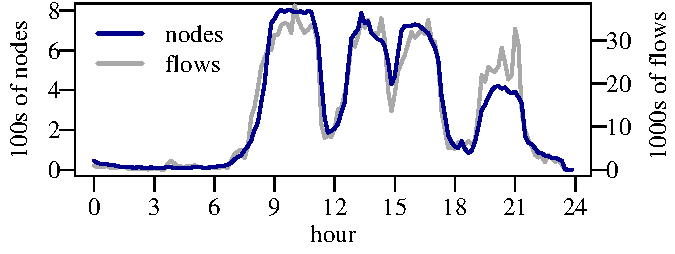
\includegraphics[width=3.5in]{nodes-flows}%
\vspace{-0.75em}%
\caption{The number of active nodes and flows over time.} 
\label{fig:nodes-flows}
\end{center}
\vspace{-2em}
\end{figure}

We do not assume or claim that the traffic found at \caps{IETF}60 is representative of conference settings in general. The observed behaviors are also unlikely to resemble those found in a typical commercial or residential setting. We have chosen this trace, however, because within it can be found behaviors resembling many different types of wireless usage cases. Figure~\ref{fig:nodes-flows} shows the wide variations in the number of active flows and nodes over the course of the trace. In the night and morning hours, the traffic patterns are similar to those one might find in a moderately trafficked business or residential area. During working group sessions, we see highly concentrated, heavy usage patterns. At the zenith of activity, over 800 users, 33 thousand flows, and 1 million packets are seen in a single 10-minute trace segment. At the nadir, a lone node sent only a single 61-byte packet over the course of 10 minutes. All levels of activity between these extremes are represented. Moreover, the mix of traffic types observed changes dramatically over the course of the day, providing a wide representation of possible blends of behavior. This heterogeneity and extreme range of behaviors makes the \caps{IETF} data set ideal for this evaluation. The variety of activity gives us greater confidence that success or failure of traffic models is not tied to any specific network condition, but is broadly and generally applicable. %For a traffic model to be truly realistic, it must be realistic across many different usage cases.

Before using the traces, it is necessary to extract application-level behavior from the trace header data. First, we split the trace into individual packet flows. A flow is a series of packets sharing the following five attributes: \caps{IP} and transport protocols (raw \caps{IP}, \caps{ICMP}, \caps{TCP}, \caps{UDP}); source and destination \caps{IP} addresses and \caps{TCP}/\caps{UDP} port numbers. Next, the quantity of application-initiated data contained in each packet is calculated. For non-\caps{TCP} packets, this quantity is simply the size of the transport-layer payload, but for \caps{TCP} the calculation is more complicated: only new data transfers, explicitly initiated by the application are counted. Data retransmitted by \caps{TCP} is disregarded, and empty \caps{ACK}s are ignored. \caps{SYN} and \caps{FIN} flags in packets (even empty ones) are counted as a single byte each, since they are explicitly signaled by the application. %After processing, we have a collection of flows, each with a sequence of timestamps and the amount of application-initiated data sent at that time.

%\begin{table}[t]
%\vspace{0.75em}
%\begin{center}
%\begin{tabular}[t]{|l|}
%\hline
%\begin{minipage}[l]{2.7in}
%\begin{small}
%\vspace{0.7em}
%\textbf{\class{Network:}}\\
\hspace*{1ex}\raisebox{1.5pt}{$\centerdot$}~collection of nodes\\
\hspace*{1ex}\raisebox{1.5pt}{$\centerdot$}~collection of flows\\
\hspace*{1ex}\raisebox{1.5pt}{$\centerdot$}~distribution of flow sizes\\
\hspace*{1ex}\raisebox{1.5pt}{$\centerdot$}~distribution of flow-source counts\\
\hspace*{1ex}\raisebox{1.5pt}{$\centerdot$}~distribution of flow-destination counts\\
\hspace*{1ex}\raisebox{1.5pt}{$\centerdot$}~distribution of intervals between flow start times\\
\hspace*{1ex}\raisebox{1.5pt}{$\centerdot$}~distribution of packet sizes\\
\hspace*{1ex}\raisebox{1.5pt}{$\centerdot$}~distribution of inter-packet intervals\\
[3pt]
\textbf{\class{Node:}}\\
\hspace*{1ex}\raisebox{1.5pt}{$\centerdot$}~session start time\\
\hspace*{1ex}\raisebox{1.5pt}{$\centerdot$}~collection of source flows\\
\hspace*{1ex}\raisebox{1.5pt}{$\centerdot$}~collection of destination flows\\
\hspace*{1ex}\raisebox{1.5pt}{$\centerdot$}~distribution of flow sizes\\
\hspace*{1ex}\raisebox{1.5pt}{$\centerdot$}~distribution of intervals between flow start times\\
\hspace*{1ex}\raisebox{1.5pt}{$\centerdot$}~distribution of packet sizes\\
\hspace*{1ex}\raisebox{1.5pt}{$\centerdot$}~distribution of inter-packet intervals\\
[3pt]
\textbf{\class{Flow:}}\\
\hspace*{1ex}\raisebox{1.5pt}{$\centerdot$}~start time\\
\hspace*{1ex}\raisebox{1.5pt}{$\centerdot$}~source node\\
\hspace*{1ex}\raisebox{1.5pt}{$\centerdot$}~destination node\\
\hspace*{1ex}\raisebox{1.5pt}{$\centerdot$}~stream of packets\\
\hspace*{1ex}\raisebox{1.5pt}{$\centerdot$}~distribution of packet sizes\\
\hspace*{1ex}\raisebox{1.5pt}{$\centerdot$}~distribution of inter-packet intervals\\
[3pt]
\textbf{\class{Packet:}}\\
\hspace*{1ex}\raisebox{1.5pt}{$\centerdot$}~send time\\
\hspace*{1ex}\raisebox{1.5pt}{$\centerdot$}~payload size (bytes)\\

%%\vspace{0.6em}
%\end{small}
%\end{minipage}
%\\\hline
%\end{tabular}
%\end{center}
%\vspace{-0.5em}
%\caption{{\footnotesize{TOM}} base classes and their attributes.}
%\label{tab:properties}
%\vspace{-2em}
%\end{table}

%\subsection{The Traffic Object Model~(\caps{TOM})}\label{sec:tom}

%\begin{table*}[t]
%\begin{center}
%\small
%\noindent
\textbf{Node:}
\begin{itemize}
  \item \textit{Individual}
  \begin{itemize}
    \item each node corresponds to a specific trace node with associated trace flows
    \item session start time assigned from trace
    \item overrides all distributions with per-node versions
  \end{itemize}
  \item \textit{Nonparametric}
  \begin{itemize}
    \item generic flows assigned to nodes by sampling
    \item session start time assigned from pool of start times
  \end{itemize}
  \item \textit{Parametric}
  \begin{itemize}
    \item generic flows assigned to nodes according to BiPareto model
    \item session start time randomly chosen from viable range
  \end{itemize}
  \item \textit{Uniform}
  \begin{itemize}
    \item all nodes have average number of generic flows
    \item session start times uniformly cover viable range
  \end{itemize}
\end{itemize}
\noindent
\textbf{Flow:}
\begin{itemize}
  \item \textit{Individual}
  \begin{itemize}
    \item each flow corresponds to a specific trace flow with an associated packet trace
    \item flow size \& start time taken from trace
    \item overrides distributions of size/interval packet behaviors with flow-specific versions
  \end{itemize}
  \item \textit{Nonparametric}
  \begin{itemize}
    \item flow size is sampled from inherited distribution of flow sizes
    \item start time relative to previous session flow sampled from inherited distribution
    \item inherits distributions of size/interval packet behaviors from destination node
  \end{itemize}
  \item \textit{Parametric}
  \begin{itemize}
    \item flow size is sampled from BiPareto model fitted to inherited distribution
    \item start time relative to previous session flow sampled Lognormal fitted to inherited
    \item inherits distributions of size/interval packet behaviors from destination node
  \end{itemize}
  \item \textit{Uniform}
  \begin{itemize}
    \item all flows have size equal to inherited mean
    \item average inter-flow interval used between all flows
    \item inherits distributions of size/interval packet behaviors from destination node
  \end{itemize}
\end{itemize}
\noindent
\textbf{Packet:}
\begin{itemize}
  \item \textit{Individual}
  \begin{itemize}
    \item each packet corresponds to a specific trace packet
  \end{itemize}
  \item \textit{Nonparametric}
  \begin{itemize}
    \item packet sizes and intervals are sampled from inherited distributions
  \end{itemize}
  \item \textit{Parametric}
  \begin{itemize}
    \item packet sizes and intervals are drawn from inherited parametric distributions
  \end{itemize}
  \item \textit{Uniform}
  \begin{itemize}
    \item all packet sizes and inter-packet intervals are equal to inherited mean
  \end{itemize}
\end{itemize}

%\footnotesize\\[0.5em]
%%\raisebox{1pt}{*}Parametric models fitted to inherited empirical distributions using maximum likelihood estimation ({\scriptsize{MLE}}).
%\end{center}
%\vspace{-0.75em}
%\caption{Details of how the sub-models at each behavioral level of the {\footnotesize{TOM}} inherit, override and delegate properties.}
%\label{tab:models}
%\vspace{-1em}
%\end{table*}

%In this section, we present a generic object-oriented framework for implementing traffic generation models. This framework is called the Traffic Object Model (\caps{TOM}). It defines four levels of responsibility: network, node, flow and packet. The framework is designed so that different behaviors at each level can be naturally implemented  as classes in object-oriented programming languages. The framework automatically gains the advantages of object orientation, in particular modularity and encapsulation. Every traffic model is naturally split into separate spheres of responsibility, which constitute sub-models for the aspects of the model's behavior at each layer. Encapsulation and polymorphism of objects, allows us to mix-and-match the sub-models from different models to create new hybrid behaviors. It is trivial, for example, to produce trace-based node behavior, coupled with parametric flow behavior, and uniform packet behavior. Not all combinations of sub-models are valid, however; which classes may be combined depends on the details of each class.

%% TODO: fix-up client-server vs. source-destination terminology.

%Abstract base classes define the properties at each level that traffic models must implement.\footnote{In Java or C\#, this role may be served either by an actual abstract class or by an interface. In duck-typed languages such as Ruby or Python, no actual abstract class need exist, since type is implicitly defined by usage; if abstract classes are desired, they can be simulated by creating base classes with stub methods that throw informative exceptions upon being called.} 
%Table~\ref{tab:properties} enumerates all the properties exposed by traffic models used in this work. Future traffic models may necessitate exposing additional properties, but this list suffices to implement the models used in this paper. Concrete subclasses implement the behavior of specific traffic models at each level. A complete synthetic workload is instantiated as follows:
%\begin{enumerate}
%\item create a \class{Network} object of the appropriate subclass;
%\item the top-level \class{Network} object in turn creates a collection of \class{Node} objects and associated \class{Flow} objects;
%\item each \class{Flow} object generates a stream of \class{Packet} objects.
%\end{enumerate}
%The hierarchy of objects may be used to directly drive a simulation, or may generate configuration files that in turn drive a simulation. Our implementation does the latter, generating a collection of Qualnet configuration files and trace files specific to each workload instantiation (see \Section{simulations}).

%\subsection{Traffic Models}\label{sec:models}

%For each of the \class{Node}, \class{Flow} and \class{Packet} abstract superclasses, we define four concrete subclasses: \class{Trace}, \class{Nonparametric}, \class{Parametric}, and \class{Uniform}. The \class{Trace} classes take properties of objects directly from the behavior of the corresponding object in the original trace. The \class{Nonparametric} and \class{Parametric} classes use models of the corresponding type to randomly generate the properties of objects. The \class{Uniform} classes generate identical objects with average properties. The specific details of how each the concrete classes at each level are defined are specified in Table~\ref{tab:models}. The parameters for the fitted models used in the \class{Parametric} subclasses are estimated from the corresponding nonparametric distribution using maximum likelihood estimation. Figure~\ref{fig:trace-vs-uniform} shows visual depictions comparing trace versus uniform behavior at various levels in example scenarios.

%While the modularity of the Traffic Object Model allows us to mix and match sub-models, not all possible combinations are valid. In particular, note that the \class{Trace} classes are tied to a specific object from the underlying trace, whereas for other classes, there is no such correspondence to any specific object. Consequently, once a non-trace model has been used, trace models may not be used at the lower levels. This still leaves 40 valid composite combinations of sub-models; we only evaluate twelve of these. Composite models are abbreviated by the initials of their constituent sub-models. The fully trace-base model, \class{TTT}, serves as an experimental control. We consider \class{TTN}, \class{TTP}, and \class{TTU} in order to compare models of packet behavior. We evaluate different flow models, using the best possible model at the packet level: \class{TNN}, \class{TPN}, \class{TUN}. Similarly, we compare models for node behavior: \class{NNN}, \class{PNN}, \class{UNN}. Finally, we use the na\"ive uniform model, \class{UUU}, and the composite parametric model, \class{PPP}, proposed by {\FHC}~\cite{Hernandez06:wlan-traffic}, as external points of comparison.

\begin{figure*}[tb]
\begin{center}
\subfloat[trace node behavior]
{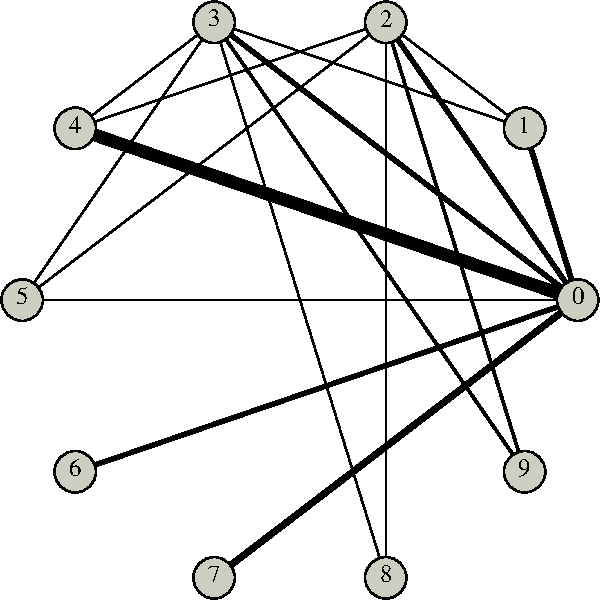
\includegraphics[width=1.392in]{flow_topology_trace}\label{fig:flow-topology-trace}}
\subfloat[uniform node behavior]
{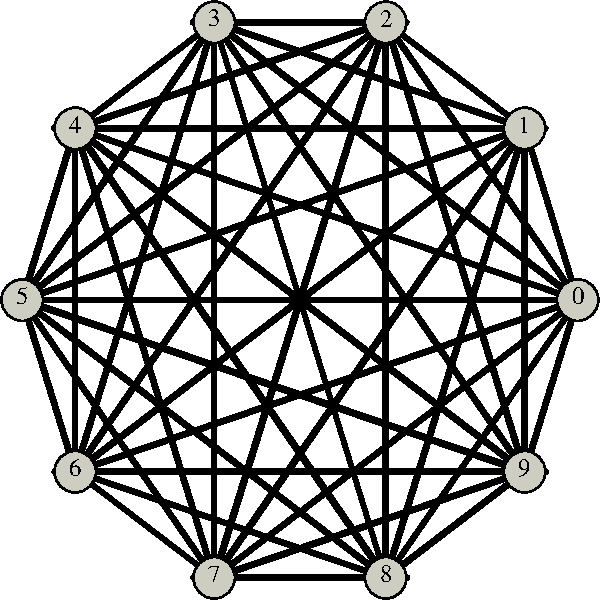
\includegraphics[width=1.392in]{flow_topology_uniform}\label{fig:flow-topology-uniform}}
\subfloat[trace flow behavior]
{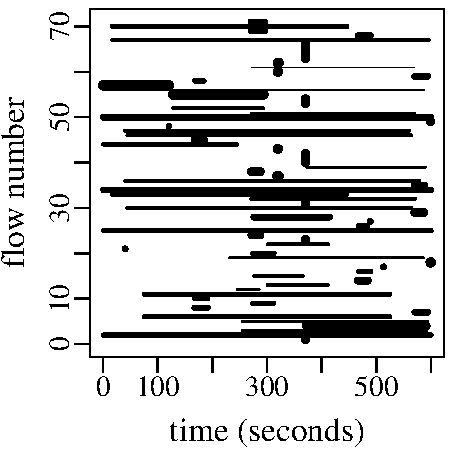
\includegraphics[width=1.392in]{flow_behavior_trace}\label{fig:flow-behavior-trace}}
\subfloat[uniform flow behavior]
{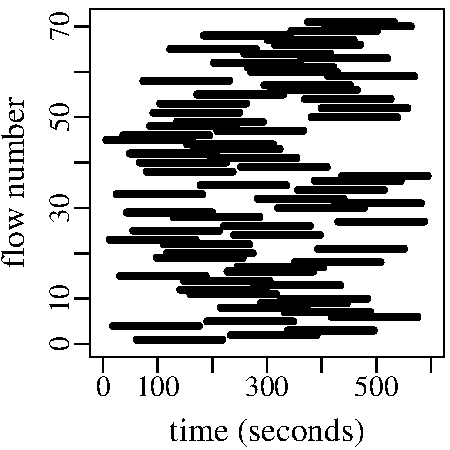
\includegraphics[width=1.392in]{flow_behavior_uniform}\label{fig:flow-behavior-uniform}}
\subfloat[packet behavior]
{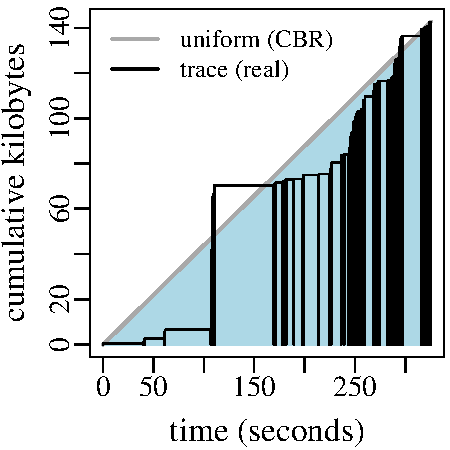
\includegraphics[width=1.392in]{flow_packet_behavior}\label{fig:packet-behavior}}
\caption{Examples illustrating trace (real) versus uniform (na\"ive synthetic) behaviors at the node, flow and packet levels. Figures \ref{fig:flow-topology-trace} and \ref{fig:flow-topology-uniform} show example node behaviors. The width of each line is proportional to the logarithm of the number of flows between the nodes it connects (zero is the Internet gateway). Uniform and trace flow behavior examples are plotted in Figures \ref{fig:flow-behavior-trace} and \ref{fig:flow-behavior-uniform}. The time axis indicates when flows start and end; the width of each flow line is proportional to the logarithm of its data rate. Figure \ref{fig:packet-behavior} compares uniform (i.e. {\footnotesize{CBR}}) packet behavior with the trace of an actual flow. In the uniform model, the cumulative data sent increases smoothly over time, whereas in the actual packet trace, the transmissions are variable both in size and in inter-packet interval, leading to a ``lumpy'' cumulative data plot.}
\label{fig:trace-vs-uniform}
\end{center}
\vspace{-2em}
\end{figure*}

%We separate traffic generation into three levels of behavior: network, flow and packet. The {network} level determines properties pertaining to nodes and their interaction. For example, it determines which nodes communicate with each other, and how frequently. This level can be viewed as assigning network nodes to the source and destination roles of flows, as well as determining per-node properties which affect lower level models. The next level of behavior determines overall properties of flows. This includes each flow's start time, duration, packet count and total data volume. Finally, the packet level of behavior determines the individual sizes of packets and the durations of intervals between their transmission. Despite the concreteness of the examples mentioned here, there are also less obvious, abstract properties that models at the network and flow levels determine. Flow models, for example, dictate the distribution of each flow's packet sizes, a property which can be used to determine individual packet sizes, but which is not itself specific to any particular packet.

%\subsubsection*{Network Behavior Models}

%We consider four models of network-level behavior. The most faithful is the ``trace'' model, which assigns each flow 

%For each level of behavior we define a spectrum of models. The gold standard of realism at each level is provided by the ``trace'' model for that level, which replicates the node, flow or packet behavior of the original trace exactly. The most rudimentary model at each level is the ``uniform'' model, which treats all entities identically---be they nodes, flows or packets. Despite being so simplistic (or perhaps because of it), the uniform behavior models are by far the most commonly for workload generation in experiments. Between these extremes on the spectrum of realism, we consider one or two models with intermediate degrees of complexity and fidelity. At the packet level, we define the ``sample'' model, which is in essence a per-flow variable bit-rate (\caps{VBR}) model: each packet's size is determined by randomly sampling a value from the packet size distribution given by the flow model; the interval until the next packet is then sampled from the given interval distribution.\footnote{Note that the uniform packet model (\textit{i.e.} {\scriptsize{CBR}}), can be considered to be a special case of the sample model where the size and time distributions are both constant.} The intermediate model at the flow level is designated as ``proportional'': the distributions of packet sizes and inter-packet intervals are taken from the trace and passed down to the packet model (which may use the actual distribution, via sampling, or simply use the mean size and intervals, to generate \caps{CBR} traffic).

%\begin{enumerate}
%\item \textbf{Network Behavior}: which nodes communicate with each other, and how frequently; \textit{i.e.} how flow end-points are mapped onto nodes in the network.
%\item \textbf{Flow Behavior}: high-level parameters for each flow, including start time, end time, packets sent, bytes sent.
%\item \textbf{Packet Behavior}: sizes of individual packets, and the intervals between their transmission.
%\end{enumerate}

%The different levels of models and variants at each level are listed and described in Table~\ref{tab:traffic-models} and illustrated with specific examples in Figure~\ref{fig:traffic-models}.

% TODO: more here on models...
% TODO: rewrite next paragraph too...

%The three levels of behavior are orthogonal and can be varied almost independently. The exception to their independence is that the trace-based packet behavior model can only be used when the flow behavior model is also trace-based. Once flow behavior is decoupled from the actual trace, there is no natural way to preserve packet behavior. This eliminates three combinations of models and leaves nine viable behaviors, abbreviated by the first letters of their flow topology, flow behavior, and packet behavior models: \caps{TTT} (fully trace-based), \caps{TTU}, \caps{TUU}, \caps{STT}, \caps{STU}, \caps{SUU} (entirely synthetic, sink topology), \caps{UTT}, \caps{UTU}, \caps{UUU} (entirely synthetic, uniform topology).

\subsection{Performance Metrics}\label{sec:metrics}

We have selected seven performance metrics at the application, network, and link layers of the protocol stack:
\begin{enumerate}
\setlength{\itemsep}{0em}
\item \textbf{Application:} average end-to-end delay, average jitter, total received throughput.
\item \textbf{Network:} \caps{AODV} control overhead (\caps{RREQ/RREP/RERR}), routing queue drop rate.
\item \textbf{Link (\caps{MAC}):} control overhead (\caps{RTS/CTS/ACK}), packet retransmission rate.
% TODO: are we actually using RTS/CTS?
\end{enumerate}
These metrics are commonly used to evaluate the performance of wireless protocols.%For each of the 144 10-minute trace segments, we have run simulations using each of the nine traffic models, for a total of 1,296 simulations.
%Unfortunately, not all of the simulations were able to run to completion. In some scenarios, the number of nodes and flows caused Qualnet to simply fail. We were, however, able to get complete results for 72.5\% of the simulations, providing a clear view of overall trends.\!\footnote{That 27.5\% of simulations did not finish may seem like a cause for concern, but it does not in fact invalidate our results. The simulations that did not finish are those for which the number of flows and nodes overwhelmed the capacity of the simulator. Qualnet cannot simulate more than circa 650 nodes sending 35,000 flows. While it would be of great interest to examine results for these large-scale scenarios, they are essentially useless for comparison to other simulations studies: other studies do not simulate this quantity of nodes and flows precisely because even the best existing simulators do not support it. Once the simulators become more scalable and robust, our analysis can be extended to these scenarios as well.}

\subsection{Simulations}\label{sec:simulations}

We use the Qualnet wireless network simulator (version 4.0.1) to perform our experiments. We simulate a stationary multi-hop 802.11g network using the Ad hoc On-demand Distance Vector (\caps{AODV}) routing protocol~\cite{rfc:aodv}, with nodes placed randomly in a square field with sides of 150 meters.
In addition to the active nodes corresponding to trace \caps{IP}s, half as many passive ``infrastructure'' nodes are added to each simulation: these nodes initiate no data and simply serve as additional network relays. Our simulations resemble multi-hop mesh networks of the kind that are increasingly studied and deployed for delivery of broadband access in residential, corporate and conference settings. We do not attempt to reproduce the physical environment of the original wireless network, nor do we simulate mobility. The only aspect of the original network's behavior that is reproduced is the total pattern of network-wide traffic.

There are a number of potential objections to this approach. We use single-hop trace data to drive multi-hop simulations; the physical environment, node mobility, handover behavior, and closed-loop dynamics of the original wireless setting are not faithfully reproduced. One must keep in mind, however, that the goal of this research is \textit{not} to understand the conditions of the original network. Rather, we are using the traffic behaviors observed as examples to help us better understand how different types of workload can affect performance metrics. In particular, we aim to understand how real workload compares with common synthetic traffic models. Of course, the reason for such objections is that networking researchers understand that the many aspects of behavior interact with each other in a complex and nearly inextricable manner. However, before we can hope to understand the interaction between workload and other features affecting network behavior, we must study traffic patterns alone, and learn to model them with reasonable accuracy in the absence of additional complicating factors. Accordingly, in this study, we detach application level traffic patterns from the other factors influencing network conditions, and study them in isolation.

The 24-hour trace is split into 144 10-minute segments, each of which serves as the basis for a set of simulations using different traffic models. The traffic models range from a completely realistic trace-driven model, to a standard \caps{CBR} traffic model. Various partially synthetic intermediate models, described in \Section{traffic-models}, are simulated to study the impact of different aspects of traffic behavior on network performance. To preserve the fairness of the performance comparison, we keep as many features as possible constant across different traffic models. The traffic generated by each synthetic model preserves as many characteristics from the original trace as possible, within the constraints of the model. Moreover, the following features are preserved across all models: the numbers of wireless nodes, the number of flows, the number of application-initiated data units sent, the total bytes of application data sent, and the average flow duration (and therefore the average data rate).

We have modified the standard Qualnet distribution in the two significant ways. First, In our previous work~\cite{Karpinski07:realism,Karpinski07:cbr-failure}, we approximated full-duplex \caps{TCP} with a pair of \caps{UDP} flows. For this work, we have implemented a new Qualnet application driver that allows trace-driven full-duplex \caps{TCP} flows. This allows us to accurately reproduce the full dynamics of \caps{TCP} feedback. Moreover, raw \caps{IP} and \caps{UDP} flows are implemented using the same code, guaranteeing that all traffic is simulated uniformly and that all performance metrics are aggregated in the same manner. The second modification is that we have instrumented Qualnet to collect \caps{IP} performance metrics in strict adherence to the recommendations of the \caps{IETF} working group recommendations~\cite{rfc:ip-metrics,rfc:jitter}.

\subsection{Measures of Error}\label{sec:error-measures}

The simulations described in \Section{simulations} provide us with the raw data to compare performance metrics for synthetic traffic models with those for real traffic traces. To assess the realism of these models, however, we need a measure of how inaccurate the synthetic performance values are when compared to the real values. Let $x$ be the value of a performance metric using real traffic, and $y$ the value of the same metric using an alternate traffic model, $\M$. Some common measures of error are the difference [$y-x$], the ratio [$y/x$], and the standard error [$(y-x)/x$]. These are all reasonable measures of error; but which is most appropriate for assessing the realism of performance metrics? Instead of picking one arbitrarily, we will first consider the properties that an ideal error function should have, and then use those properties to determine the best measure of error. Moreover, we will show that the unique measure of error that exhibits these ideal properties is the  \textit{log-ratio} of metric values:
\begin{align}
\log(y/x)=\log(y)-\log(x).
\end{align}
In this discussion, $E(x,y)$ is a generic error function applied to the synthetic value, $y$, with respect to the real value, $x$.

The first property that an error function should have is  \textit{insensitivity to common factors}. That is, if both values are scaled by the same constant, the error should be unaffected:
\begin{align}
\label{eqn:normalization-invariance}
\forall\: x,y,c: E(x c,y c) &= E(x,y)
\end{align}
There are three major motivations for this requirement:
\begin{enumerate}
\item Changing units should not affect error values.
\item Error values for ``large'' and ``small'' scenarios should be directly comparable. Scenarios with large $x$ values will naturally have larger raw differences between $x$ and $y$. This requirement allows scenarios of different scales to be compared fairly and without bias.
\item Changing between metrics that differ by a known constant for each scenario should not affect error values.
\end{enumerate}
The last point is best illustrated by an example. Consider two closely related performance metrics: average throughput, $t$, and total bytes received, $r$. Suppose that there are $f$ flows in a given scenario with average duration, $d$. Since $t =r/fd$, the metrics $t$ and $r$ contain the same information---they differ only by a known constant in each simulation scenario. Equation~\ref{eqn:normalization-invariance} ensures that the errors of these metrics are the same:
\begin{align}
E(t^\TTT,t^\M)
	= E\left({\frac{r^\TTT}{fd},\frac{r^\M}{fd}}\right)
	= E(r^\TTT,r^\M).
\end{align}
The difference measure does not satisfy Equation~\ref{eqn:normalization-invariance}, but the ratio, standard error, and log-ratio error measures all do.

The second property that an ideal error function should have is  \textit{additivity of compounded errors}. If two independent causes of error each induce some factor of misrepresentation, then the combined error should be the sum of the errors caused by each factor separately:
\begin{align}
\label{eqn:linear-compounding}
\forall\: x,c_1,c_2:
	E(x,x c_1 c_2) &= E(x,x c_1) + E(x,x c_2).
\end{align}
This property allows us to compare error values meaningfully across different traffic models. For example, if flow topology and packet behavior affected some performance metric independently with no interaction effects, we would expect that
\begin{align}
E(x^\TTT,x^\UTU) \approx E(x^\TTT,x^\TTU) + E(x^\TTT,x^\UTT).
\end{align}
If these two values differ significantly, there must be some interaction between the two levels of behavior that introduces more error than can be explained by each separately. Without the property of additivity given in Equation~\ref{eqn:linear-compounding}, such a comparison would not be possible or meaningful.

Additivity of compounded errors also implies two desirable properties that are easily derived from Equation~\ref{eqn:linear-compounding}. It forces the error of an accurate representation to be zero: $E(x,x) = 0$. It also forces underestimation and overestimation to be treated symmetrically. The error of underestimating by some factor is opposite but equal to overestimating by the same factor:
\begin{align}
E(x,x/c) = - E(x,xc).
\end{align}

It is easily verified that the difference, ratio, and standard error measures do not satisfy Equation~\ref{eqn:linear-compounding}, and the difference, as noted, does not satisfy Equation~\ref{eqn:normalization-invariance}. The log-ratio is the only metric presented that satisfies both conditions. Moreover, it can be proved that $\log(y/x)$ is the \textit{only} differentiable function that satisfies both (up to a constant). In the Appendix, we present a proof of this claim. Throughout the rest of the paper, we use the log-ratio to measure the error of performance metrics.
% TODO: should Appendix be capitalized?
% TODO: hyperref the Appendix for PDF.

%\subsection{Tests of Statistical Equivalence}\label{sec:statistical-equivalence}

%%\begin{sidewaysfigure*}
%%%\begin{centering}
%%\noindent
%%\subfloat[Application: Average Jitter]
%%{\includegraphics[width=4.6in]{Application-Average-Jitter}
%%\label{fig:Application-Average-Jitter}}
%%\subfloat[Application: Average Delay]
%%{\includegraphics[width=4.6in]{Application-Average-Delay}
%%\label{fig:Application-Average-Delay}}
%%\subfloat[Application: Received Throughput]
%%{\includegraphics[width=4.6in]{Application-Received-Throughput}
%% \label{fig:Application-Received-Throughput}}
%%\subfloat[Network: Control Overhead]
%%{\includegraphics[width=4.6in]{Network-Control-Overhead}
%% \label{fig:Network-Control-Overhead}}
%%\subfloat[Network: Packet Drop Rate]
%%{\includegraphics[width=4.6in]{Network-Packet-Drop-Rate}
%% \label{fig:Network-Packet-Drop-Rate}}
%%\subfloat[Network: \caps{RREQ}s Initiated]
%%{\includegraphics[width=4.6in]{Network-RREQs-Initiated}
%% \label{fig:Network-RREQs-Initiated}}
%%\subfloat[Link (MAC): Control Overhead]
%%{\includegraphics[width=4.6in]{MAC-Control-Overhead}
%% \label{fig:MAC-Control-Overhead}}
%%\subfloat[Link (MAC): Retransmissions]
%%{\includegraphics[width=4.6in]{MAC-Retransmissions}
%% \label{fig:MAC-Retransmissions}}
%%\subfloat[Link (\caps{MAC}): Retransmission Failures]
%%{\includegraphics[width=4.6in]{MAC-Retransmission-Failures}
%% \label{fig:MAC-Retransmission-Failures}}
%%\hspace{0.035in}
%%\begin{minipage}[t]{4.545in}
%%\vspace{-2em}
%%\caption{Box-and-whisker plots of log-ratio error values for all metrics and traffic models. The lower axis indicates the log-ratio, while the upper axis shows raw ratio values. Each box contains the central majority of log-ratio values: the left and right bounds are at the $25^\text{th}$ and $75^\text{th}$ percentiles. The dark middle line indicates the median value, while the diamond marks the mean. The whiskers (dotted lines) extend to the furthest non-outlier values, while the points beyond that are outliers. The notches in the middle show a $95\%$ confidence interval for the actual underlying median value; if two notches do not overlap, they are very unlikely to have the same median. Numbers to the right are $p$-values for the median, mean, and 3-mean tests, respectively; $p$-values above $\alpha=0.05$ appear in bold.}
%%\label{fig:boxplots}
%%\end{minipage}
%%%\end{centering}
%%\end{sidewaysfigure*}

%In this section, we consider the values of performance metrics as random variables, drawn from unknown distributions. We present three tests for the statistical equivalence of the metric values induced by synthetic and real traffic. Let $\M$ be a traffic model as before and let $\X$ be a performance metric. Let $X_k^\M$ be a random variable representing the value of $\X$ in the $k^{\text{th}}$ scenario using the traffic model $\M$. If the distribution of $X_k^\M$ is the same as that of $X_k^\TTT$, then both the median and mean values of the log-ratio $R_k^\M=\log(X_k^\M/X_k^\TTT)$ should be zero. The first two tests check the plausibility of precisely these hypotheses. The third test separates small, medium, and large simulation scenarios, and test their means separately to catch any size-dependent performance bias.

%\textbf{The Median Test.} If $\M$ induces realistic performance, then the median of each log-ratio variable, $R_k^\M=\log(X_k^\M/X_k^\TTT)$, should be zero. The $k^\text{th}$ indicator variable is defined as
%\begin{align}
%	I_k^\M = \begin{cases}
%		0 & \text{if $R_k^\M < 0$,} \\
%		1 & \text{if $R_k^\M \ge 0$.}
%	\end{cases}
%\end{align}
%If the median value of $R_k^\M$ is truly zero, then $I_k^\M$ is a Bernoulli variable with probability parameter $p=\frac{1}{2}$. The variables $I_k^\M$ are all independent since they come from separate simulations, and cannot affect each other's outcomes. Therefore, the sum $S_n^\M = \sum_{k=1}^n {I_k^\M}$ should follow a binomial distribution of $n$ trials with $p=\frac{1}{2}$. The median test applies the exact binomial cumulative distribution function (\caps{CDF}) % TODO: cite this.
% for $n$ and $p$ to the observed value of $S_n^\M$, yielding a $p$-value: the probability that such an extreme value would occur by chance under the hypothesis that the median of each $R_k^\M$ is zero. % TODO: fix the wording here.

%%\begin{figure*}
%%\begin{centering}
%%\subfloat[App. Average Jitter: {\footnotesize{STU}}]
%%{\includegraphics[width=1.75in]{application-average-jitter-stu}%
%%\label{fig:application-average-jitter-stu}}
%%\subfloat[Net. Packet Drop Rate: {\footnotesize{UTU}}]
%%{\includegraphics[width=1.75in]{network-packet-drop-rate-utu}%
%%\label{fig:network-packet-drop-rate-utu}}
%%\subfloat[Net. Packet Drop Rate: {\footnotesize{STU}}]
%%{\includegraphics[width=1.75in]{network-packet-drop-rate-stu}%
%%\label{fig:network-packet-drop-rate-stu}}
%%\subfloat[Link Retrans. Failures: {\footnotesize{SUU}}]
%%{\includegraphics[width=1.75in]{mac-retransmission-failures-suu}%
%%\label{fig:mac-retransmission-failures-suu}}
%%\caption{Scatter plots of various metrics for an alternate traffic model ({\footnotesize{STU}}, {\footnotesize{UTU}}, {\footnotesize{SUU}}) versus real trace traffic~({\footnotesize{TTT}}). Each data point represents a pair of matched simulations: the $x$-coordinate is the metric value for trace traffic, the $y$-coordinate is the metric value for the synthetic model. Scenarios are plotted according to the amount of flows in their trace segment: the bottom third with filled dots; the middle third with circles; the top third with squares.}
%%\label{fig:scatterplots}
%%\end{centering}
%%\vspace{-1em}
%%\end{figure*}

%\textbf{The Mean Test.} We use Lyapunov's generalization of the Central Limit Theorem (\caps{LCLT}) to test the hypothesis that the mean of each $R_k^\M$ is zero. We present the theorem and its application to the series $R_k^\M$ in the Appendix. Here we simply present the resulting test statistic and its usage. If the mean of each $R_k^\M$ is zero, then \caps{LCLT} implies that the test statistic
%\begin{align}
%\hat{Z}_n^\M &= \frac{\sum_{k=1}^n{R_k^\M}}{\sqrt{\sum_{k=1}^n{(R_k^\M)^2}}}
%\end{align}
%converges to a standard normal distribution for large values of $n$, where $n$ is the number of simulated scenarios. In this case, $n=144$, which is fairly large by traditional statistical standards. The $p$-value of the mean test is given by applying the standard normal \caps{CDF} to the test statistic, $\hat{Z}_n^\M$.

%\textbf{The 3-Mean Test.} Performance behavior in scenarios with a large number of nodes or flows is often very different from behavior in small scenarios. In some cases, $R_k^\M$ is skewed positively for one group, but negatively for another. In such cases, $R_k^\M$ can pass the median and mean tests even though behavior in each case is unrealistic. To catch such situations, we split the simulations into three groups by the number of flows: the lower, middle, and upper thirds. The 3-mean test simply applies the mean test to each of these groups separately and uses the minimum $p$-value of the three. This reduces the power of the test, since each group is smaller, but can catch cases where the error has size-dependent biases that cancel out on average.

\section{Results}\label{sec:results}

\begin{sidewaysfigure*}
%\begin{figure*}[htb]
\subfloat[\textbf{Application:} Average End-to-End Delay]%
{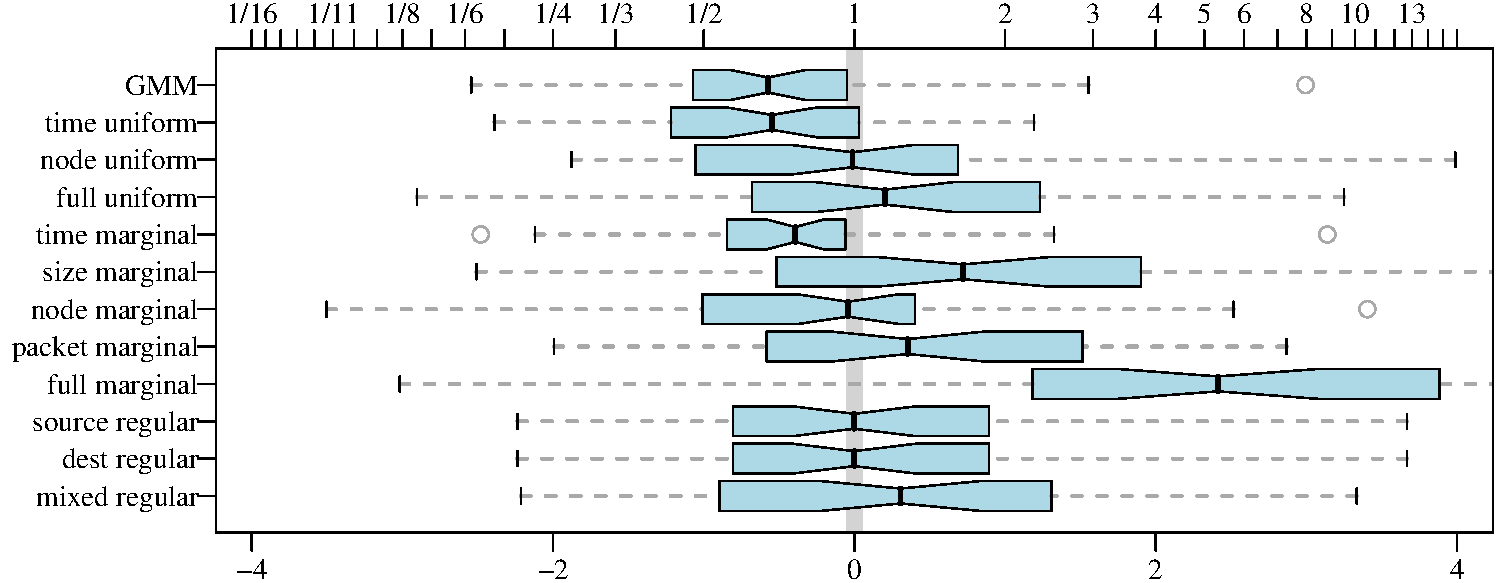
\includegraphics[width=4.6in]{plots/Application/delay.pdf}}
\subfloat[\textbf{Application:} Average Received Throughput]%
{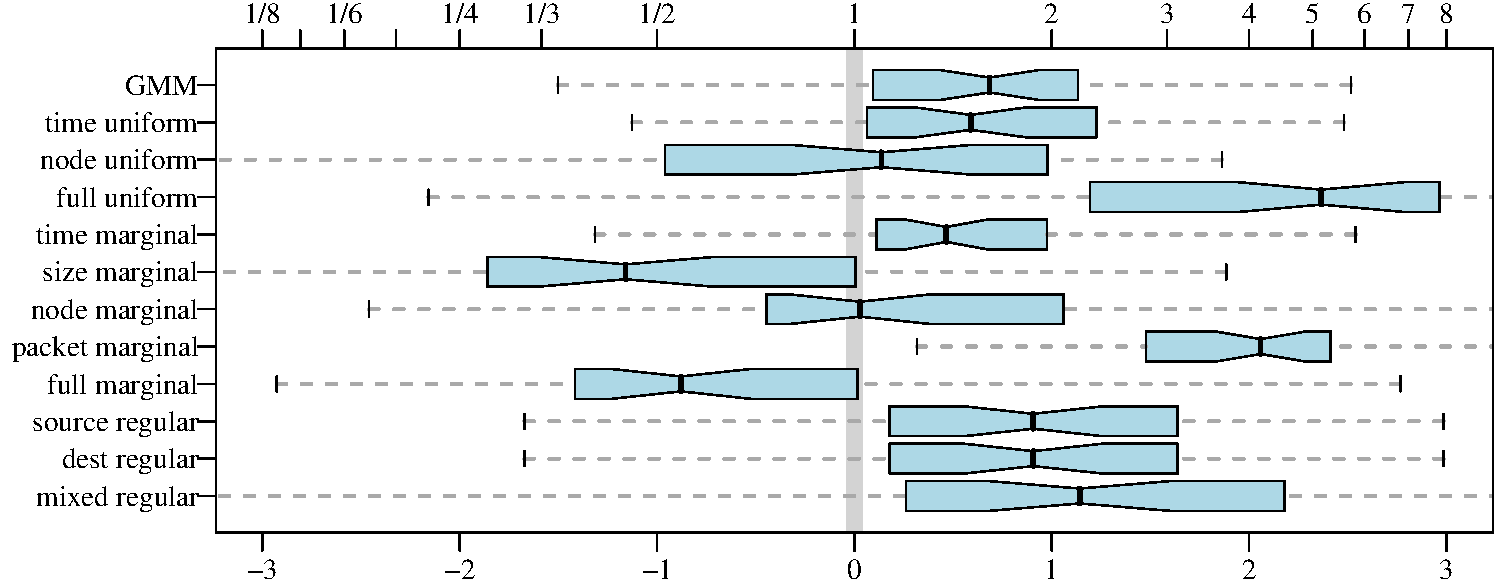
\includegraphics[width=4.6in]{plots/Application/throughput.pdf}}
\subfloat[\textbf{Application:} Total Received Packets]%
{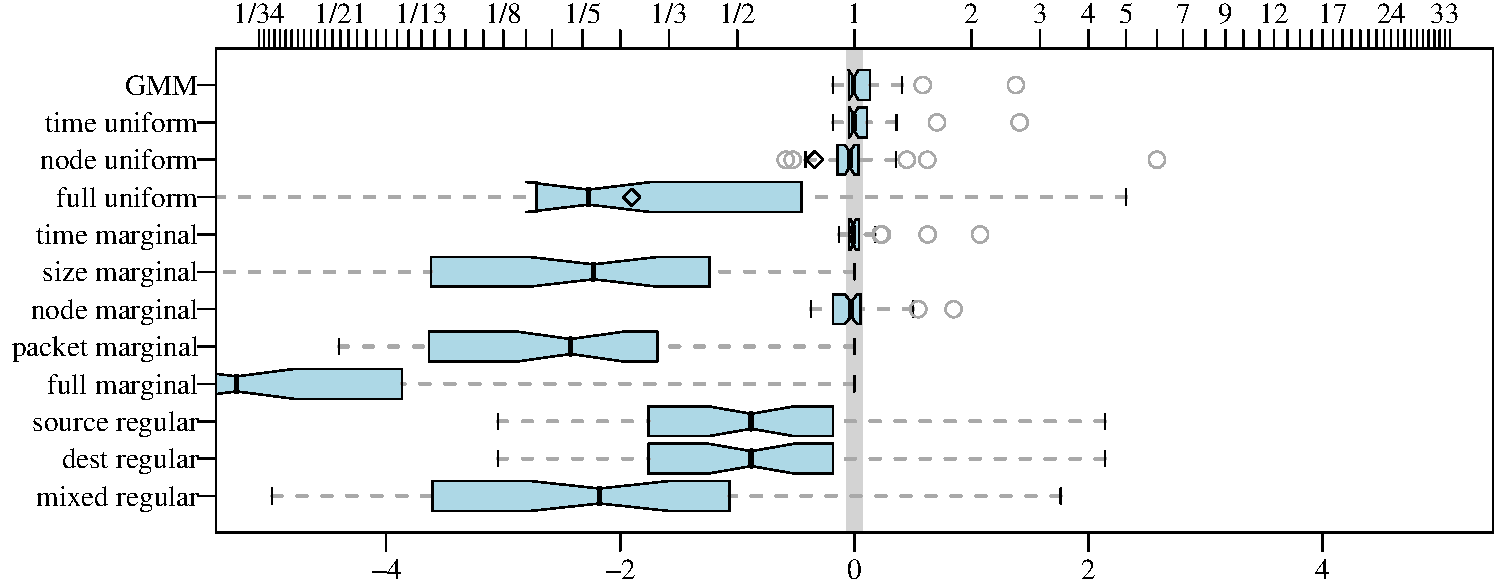
\includegraphics[width=4.6in]{plots/Application/total_recv_packets.pdf}}
\subfloat[\textbf{Network:} AODV Control Overhead]%
{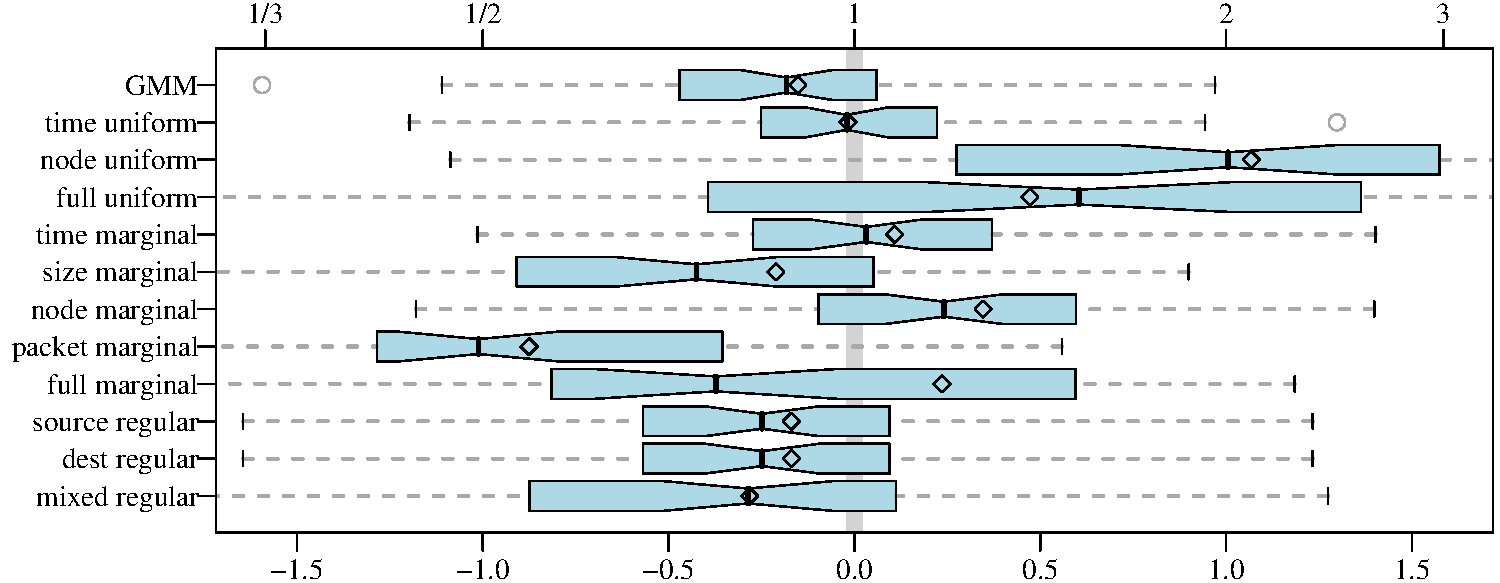
\includegraphics[width=4.6in]{plots/Network/control_packets.pdf}}
\subfloat[\textbf{Network:} Packets Dropped in Routing Queue]%
{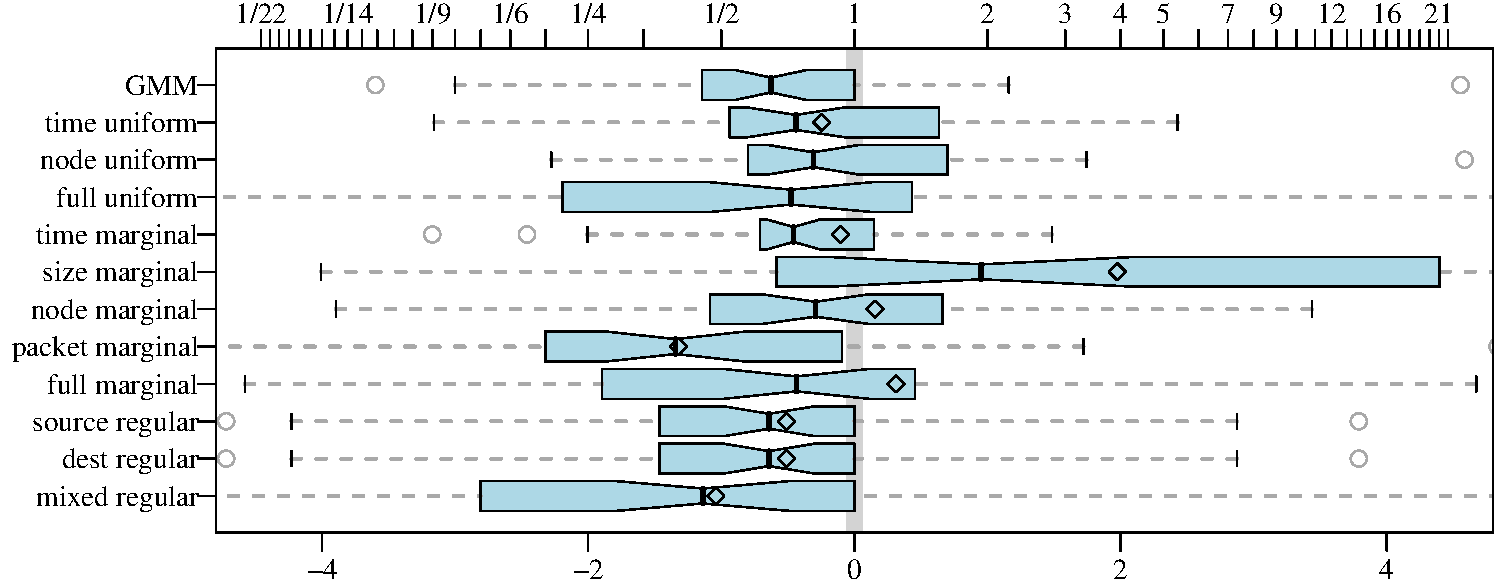
\includegraphics[width=4.6in]{plots/Network/dropped.pdf}}
\subfloat[\textbf{Link:} 802.11 Control Overhead]%
{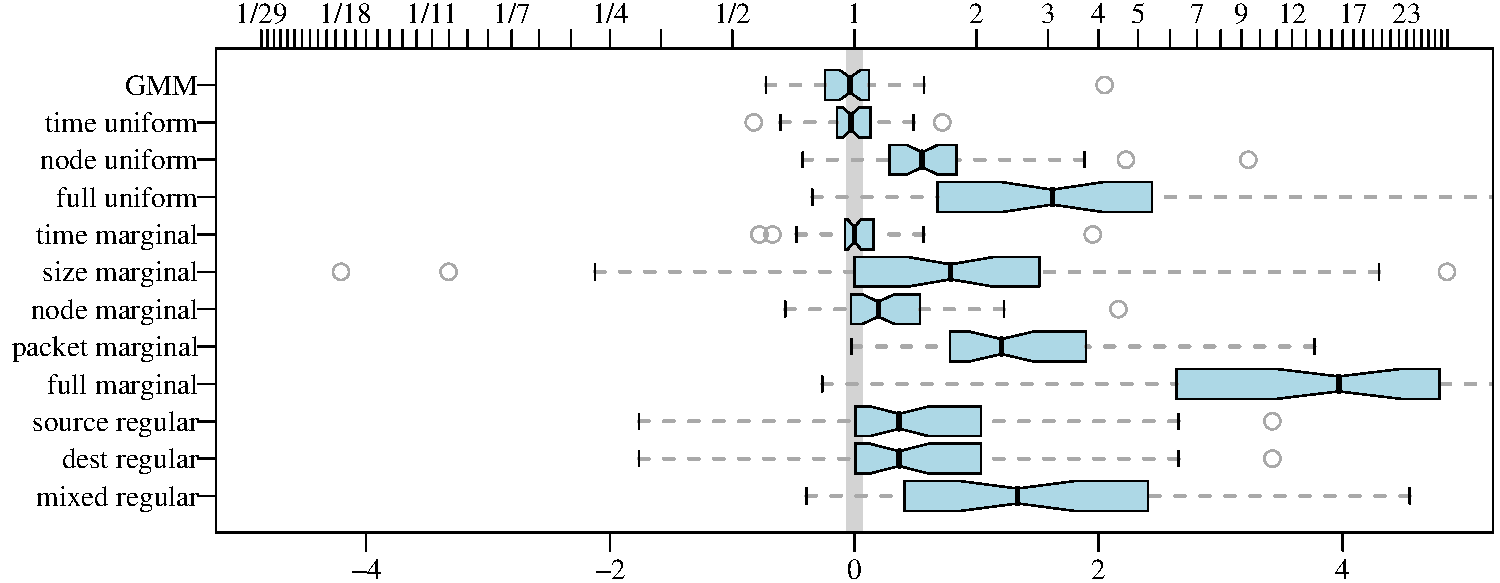
\includegraphics[width=4.6in]{plots/Link/overhead.pdf}}%
\caption{Box-and-whisker plots of log-ratio error values for all metrics and traffic models. The lower axis indicates the log-ratio, while the upper axis shows raw ratio values. Each box contains the central majority of log-ratio values: the left and right bounds are at the $25^\text{th}$ and $75^\text{th}$ percentiles. The dark middle line indicates the median value, while the diamond marks the mean. The whiskers (dotted lines) extend to the furthest non-outlier values, while the points beyond that are outliers. The notch in the middle of each bar indicates a $95\%$ confidence interval for the true underlying median value; if two notches do not overlap, they are very unlikely to have the same median.}
\label{fig:box-plots}
%\vspace{-1.25em}
%\end{figure*}
\end{sidewaysfigure*}

Our simulation results are summarized in Figure~\ref{fig:box-plots}. Each subfigure shows a single performance metric. The distribution of errors for each traffic model is visualized with a box-and-whisker plot. These plots allow immediate assessment of realism: a good traffic model should have log-ratio values that are tightly clustered around the center, with a small, evenly balanced box. Additionally, the mean and median markers should be close to the center. 

The primary result is that the General Matrix Model~(\caps{GMM}) is sufficiently realistic. It accurately reproduces important performance metrics at all levels of the protocol stack in simulation. This only moves us a step closer to being able to generate realistic, completely synthetic workloads, since the \caps{GMM} in these comparisons  derives almost all of its behavior directly from the trace. However, it means that we have effectively reduced the problem of generating realistic workload to the problem of classifying and understanding what sorts of traffic matrices occur in real workloads. Moreover, we can express a vast array of different approaches to traffic modeling simply and uniformly using matrix operations.

\section{Discussion}\label{sec:discussion}

What are the ramifications of these results? The discovery that the most commonly used traffic model for wireless networks drastically misrepresents important performance metrics may shed some light on the lack of trust in results from wireless simulations. It is now well established that network usage behavior---both mobility, and, with this research, traffic patterns---have an impact on network performance that cannot be ignored. Even experimental deployments cannot avoid the need for more realistic traffic workload models. While using a real, physical network successfully sidesteps simulation problems below the application layer, without realistic traffic models, reliable, meaningful performance predictions remain beyond our reach.

\subsection{Generality of Results}

% TODO: talk about other synthetic models not considered here.
% The point of our analysis is not to show that no synthetic models can be accurate, but rather, that the commonly used models, and obvious variations thereof, are not accurate.

The most significant limitation on the generality of this analysis is that it is based entirely on a single data set from \caps{IETF}60---albeit a large and varied one. It is possible that traffic in this trace happens to produce network performance that is unusually dissimilar to standard traffic models. This data set, however, represents a highly heterogeneous collection of network usage behaviors, from slow and steady off-peak usage, to extremely heavy peak usage: over 800 users, 33 thousand flows, and 1 million packets in a single 10-minute trace segment. Despite the broad variety of behaviors, the results are consistent: in all types of usage scenarios, simplistic traffic models, like uniform \caps{CBR}, systematically skew important performance measurements at all levels of the network. While the precise results for other data sets might differ, it is very unlikely that \caps{CBR} traffic models will happen to accurately reproduce realistic performance in other experiments. This paper provides strong evidence that better traffic models are needed for performance evaluations.

\subsection{Towards Realistic Models of Wireless Workload}

What would better traffic models look like? How can we create them? One possible approach is to use actual traffic traces as we have done. This approach is unsatisfactory, however, because it provides the experimenter with almost no control over experiments. Synthetic models have parameters, which can be tweaked as necessary---adjusting, for example, the number of active nodes in a simulation, without affecting other parameters. Traffic traces, on the other hand, must be used without significant alteration if they are to actually provide the desired realism. %The ``messiness'' of the performance comparison from trace data in Figure~\ref{fig:mac-control-overhead-cmp} illustrates why using traces directly is not ideal: each data point differs not only in the number of nodes shown on the $x$-axis, but also in other dimensions, such as the number of flows and packets, and the average flow duration. The result is a highly noisy comparison, affected by many unseen parameters. Only by applying a local smoothing algorithm are trends somewhat elucidated.

Instead of using trace data directly, it should be possible to configure a synthetic traffic model based on observations from a real data set, and then run side-by-side simulations using the synthetic model and the real data, producing statistically equivalent performance results. This is precisely what our definition of sufficient realism entails. The work in this paper provides the tools to measure how close to this ideal a model is and in what areas it needs improvement. Without this feedback, any improvements in realism are purely guesswork. Our breakdown of traffic behavior into three orthogonal levels also allows the problem to be approached in smaller pieces, rather than being solved all at once.

%The next step towards better traffic models is to investigate which aspects of real traces may be altered without detrimentally affecting the resulting performance metrics. For example, to test whether a complex time-series model of packet behavior is necessary, we randomize the order of the packet sizes and/or inter-packet intervals and compare performance using these randomized traces against performance using the original traces. If the performance is unchanged, we can conclude that no complex time-series model of packet behavior is necessary: sampling the packet sizes and inter-packet intervals from empirical distributions is sufficiently realistic. If, on the other hand, the performance characteristics are altered by shuffling packets, then some time-series model of packet behavior is needed. By partially randomizing the packet order in specific ways, the exact limits of realism necessary can be found. A similar approach will allow the development of realistic models for the other levels of network usage behavior.

\section{Conclusions}\label{sec:conclusions}

%The real significance of this paper lies not in showing that the commonly used \caps{CBR} traffic model is unrealistic. Networking researchers understand that \caps{CBR} is at best a na\"ive approximation of real network traffic. Nor is the real significance that we have quantized the high degree of inaccuracy that can be induced by using this model. The real significance of this paper lies in providing an well-defined, objective measure of realism for traffic models. This has never previously existed: evaluations of realism have relied on essentially arbitrary statistical measures of similarity to real traffic. Existing traffic generators use empirical distributions of such quantities as file size, inter-connection time, packet size, or inter-packet intervals. They can only hope that reproducing these distributions as good enough. Without an external measure of accuracy, there's simply no way to know.

%attempting to showing that existing models are unrealistic, or that new models are more realistic have always focused on arbitrary statistical measures. A 

This research rigorously quantifies the impact of a variety of synthetic traffic models on performance metrics that wireless researchers use to evaluate new technologies and protocols. The first step in this assessment process was to formally define what it means for a network usage model to be sufficiently realistic. In essence, a model is considered realistic if it produces performance results that are statistically equivalent to those produced by real usage.
A well-defined, objective measure of realism for traffic models has not previously existed. Evaluations of realism have formerly relied on essentially arbitrary statistical measures of similarity to real traffic, which may or may not affect the performance metrics that researchers care about.
The definition of sufficient realism leads us to our general experimental approach: we use differential analysis comparing performance metrics derived from real traffic with those derived from synthetic traffic models. The theoretical contributions of this analysis are:
\begin{enumerate}
\item An in-depth analysis of the desirable mathematical properties of a measure of error for performance metrics.
\item Proof that the unique measure of error that satisfies these properties is the log-ratio of metric values.
\item Three rigorous tests of statistical equivalence between synthetic and real performance results.
\end{enumerate}
These analytical tools allow the evaluation of realism over a collection of drastically different usage scenarios. Evaluation over a heterogeneous collection of scenarios is essential to establishing the credibility of usage models. Moreover, these theoretical results are equally applicable to other types of usage models---for example, mobility.

On the practical side, this paper gives crucial insight into why most researchers do not trust simulation results: with the traffic models commonly used, the results are unlikely to reflect real performance. Moreover, this problem will also hamper experiments in test-bed wireless networks, so long as the same na\"ive workload models are used. The only way to address this fundamental lack of realism is to develop usage models that reproduce important performance metrics more accurately. Our theoretical results provide the tools necessary to do this. The development of better traffic models should begin with real traces, and proceed by incremental changes, checked by differential analysis.
%First, alter a small aspect of the trace, simulate, then compare. If the realism of the results is unaffected, the traffic feature altered was inessential. Otherwise, it is a feature of behavior that must be captured in a realistic traffic model.
This approach will allow the precise mapping of which aspects of traffic patterns have an impact on performance and which ones can be safely abstracted away.
% TODO: maybe cut out some of this last bit.

%\section{Acknowledgments}
%This work was funded in part through NSF Career Award CNS-0347886.

\vspace{-0.5em}
\appendix\footnotesize

\noindent
\textbf{Theorem.} The unique differentiable function satisfying Eqs.~\ref{eqn:normalization-invariance}~\&~\ref{eqn:linear-compounding} is $E(1,e) \ln(y/x)$. \textit{Proof:} Let $f(z) = E(1,z)$. Eq.~\ref{eqn:normalization-invariance} gives $E(x,y) = E(1,y/x) = f(y/x)$. Eq.~\ref{eqn:linear-compounding} gives: $f(z) = f(z/w) + f(w)$. Differentiation by $z$ yields $f'(z) = w^{-1} f'(z/w)$. In particular, if we choose $w=z$, we get $f'(z) = z^{-1} f'(1)$. Integration by $z$ gives:
$f(z) = f'(1) \int z^{-1} dz + c = f'(1) \ln(z) + c$.
By Eq.~\ref{eqn:linear-compounding}, $f(1)=0$, so $c=0$. Thus $f(e)=f'(1)\ln(e)=f'(1)$. We conclude that $f(z)=f(e)\ln(z)$, so $E(x,y) = f(y/x) = f(e)\ln(y/x) = E(1,e)\ln(y/x)$, as desired.\hfill\QED

%\vspace{1em}\noindent
%\textbf{Theorem.}~[\textit{Lyapunov's Central Limit Theorem}] Let $\{R_k\}_{k=1}^{\infty}$ be a series of independent variables with $\E{R_k}=0$. Let $s_n^2 = \sum_{k=1}^n{\E{\abs{R_k^2}}}$ and $r_n^3 = \sum_{k=1}^n{\E{\abs{R_k^3}}}$. For each $n$, let $Z_n$ be the normalized mean of $\{R_k\}_{k=1}^n$: $Z_n = \sum_{k=1}^n{R_k/s_n}$. If $\lim_{n\to\infty} {r_n/s_n} = 0$, then $\lim_{n\to\infty}{Z_n} \sim \mathcal{N}(0,1)$ (the standard normal distribution). (See~\cite{Feller68} page 229.)

%\vspace{1em}
%To apply the LCLT to the series $R_k^\M=\log(X_k^\M/X_k^\TTT)$, we must show that under the null hypothesis, the assumptions of the theorem are satisfied by this series. First, the null hypothesis, implies that $\E{R_k}=0$. Variables from separate simulations are independent since they cannot influence each other's values. Formally, $\Pr\left(X_k\middle|X_j\right)=\Pr\left(X_k\right)$. Therefore the log-ratios are also independent for different $k$. The last requirement is that $\lim_{n\to\infty}{r_n/s_n}=0$. To verify this, we use the estimators $\hat{s}_n^2=\sum{\abs{R_k^2}}$, and $\hat{r}_n^3=\sum{\abs{R_k^3}}$. When $\hat{r}_n/\hat{s}_n$ are plotted on a log-log scatter plot, with $n$ increasing up to the number of simulations, they asymptotically approach a downwardly sloped line as $n$ grows. Thus $\lim_{n\to\infty}{\ln(\hat{r}_n/\hat{s}_n)/\ln(n)}=c<0$. This implies that $\lim_{n\to\infty}{\ln(\hat{r}_n/\hat{s}_n)}=-\infty$, and therefore $\lim_{n\to\infty}{r_n/s_n}=\lim_{n\to\infty}{\hat{r}_n/\hat{s}_n}=0$. This test for the convergence of $r_n/s_n$ is applied to each model and metric pair. %The asymptotic approach of the ratio $\hat{r}_n/\hat{s}_n$ to a downwardly sloped line is verified visually and by comparison to a fitted regression line.

%\vfill

%\pagebreak
% Hernandez06:dissertation: ``complete methodology for reproducing the traffic observed on a network link in a closed-loop manner, and proposed a number of metrics for studying the realism of the generated traffic.''
\bibliography{IEEE,references}

\end{document}

